%% 美赛模板:正文部分

\documentclass[12pt]{article}  % 官方要求字号不小于 12 号,此处选择 12 号字体

% 本模板不需要填写年份,以当前电脑时间自动生成
% 请在以下的方括号中填写队伍控制号
\usepackage[209050796]{easymcm}  % 载入 EasyMCM 模板文件
\problem{A}  % 请在此处填写题号
\usepackage{mathptmx}  % 这是 Times 字体,中规中矩 
%\usepackage{mathpazo}  % 这是 COMAP 官方杂志采用的更好看的 Palatino 字体,可替代以上的 mathptmx 宏包

\title{Estimated Annual Size of Claims Arising from Fire}  % 标题

% 如需要修改题头(默认为 MCM/ICM),请使用以下命令(此处修改为 MCM)
%\renewcommand{\contest}{MCM}

% 文档开始
\begin{document}

% 此处填写摘要内容
\begin{abstract}
    The aim of this study is to construct a mathematical model based on Markov chains to predict \
    the total size of claims paid by insurers in the UK (and specifically England) due to fires in \
    the coming year. We split the regions of England into\ 
    \emph{"South West", "South East", "London", "East of England", "East Midlands", "Yorkshire and The Humber", "North West", "West Midlands", "North East"} \ 
    in order to obtain more refined predictions. First, we used house price data as a proxy for the \
    size of the claim per fire, assuming a fixed ratio of damage to the size of the claim per fire. \
    We then fitted the house price data with a log-normal distribution to obtain the distribution of \
    each claim size. Next, we modelled the number of fires using a Poisson distribution with a high \
    probability estimate. Finally, we use Monte Carlo simulations to estimate the size of the annual \
    fire loss. Our model takes into account two key factors, the number of fires and the size of claims \
    per fire, and provides insurers with an effective tool for predicting and managing fire insurance risk. \
    However, there are some assumptions and limitations to our model, such as our assumption of a fixed ratio \
    of losses to claim sizes per fire, which may not be entirely accurate in real life situations. \
    Future research could further improve this model to increase its predictive accuracy and usefulness. \\
    All data is taken from GOV.UK, the official website of the UK government.\\

    % 美赛论文中无需注明关键字。若您一定要使用,
    % 请将以下两行的注释号 '%' 去除,以使其生效
    \vspace{5pt}
    \textbf{Keywords}: Monte Carlo simulations, Log-normal distribution, Poisson distribution

\end{abstract}

\maketitle  % 生成 Summary Sheet
\tableofcontents  % 生成目录


% 正文开始
\section{Introduction}
\subsection{Problem Background}
Forecasting fire insurance claims is an important part of risk management for insurance companies. \
Accurate forecasting can help insurers set appropriate insurance rates to ensure their long-term \ 
financial stability. However, forecasting fire insurance claims $S=\sum^{N}_{i=1}X_i$ involves two important issues: \ 

\begin{itemize}
    \item the Number of Fires, which is $N$
    \item the Size of Claims per Fire, which is $X_i$
\end{itemize}

First, the number of fires is a random variable whose distribution can be influenced by many factors\ 
such as climatic conditions, building quality and safety measures. To simplify the problem, we assume\ 
that the number of fires follows a Poisson distribution. This assumption is based on the fact that the\ 
Poisson distribution is often used to model the number of events occurring in a given period of time. \textsuperscript{\cite{poisson}}

Secondly, the amount claimed per fire is also a random variable whose distribution can be influenced\ 
by many factors, such as the severity of the fire, the insurance coverage of the house, etc. As we do\
not have direct access to claims data for each fire, we use house price data as a proxy for the amount\
claimed per fire and assume that\
\textbf{the ratio of house price to the amount claimed per fire, which we called  $ \rho $}, is fixed.\
This assumption is based on our observation that house prices are typically proportional to the\
value of the house and the amount of potential loss.

\subsection{Our work}

Based on these assumptions, our solution process is as follows:    

\begin{enumerate}[\bfseries 1.]
    \item We fit the house price data with a lognormal distribution to obtain the\ 
    distribution of the amount of each claim.\textsuperscript{\cite{house1, house2}}
    \item We then use\ 
    a Poisson distribution with maximum likelihood estimation to model the number of fires.
    \item Finally, we use Monte Carlo simulations to estimate the amount of fire losses each year.
\end{enumerate}

This process covers\
two key factors, the number of fires and the amount of claims per fire, and provides insurers with an\ 
effective tool for predicting and managing fire insurance risk.

\section{Preparation of the Models}

\subsection{Notations}
The primary notations used in this paper are listed in Table \ref{tb:notation}.

% 三线表示例
\begin{table}[!htbp]
\begin{center}
\caption{Notations}
\begin{tabular}{cl}
	\toprule
	\multicolumn{1}{m{3cm}}{\centering Symbol}
	&\multicolumn{1}{m{8cm}}{\centering Definition}\\
	\midrule
	$S$&Total Losses to Cover All Claims\\
	$N$&Number of Claims during a year\\
	$X_i$ &Size of the i-th Claim\\
    $A_i$ &House Price without Inflation\\
    $a_i$ &House Price with Inflation\\
    $CPI$ &Consumer Prices Index \\
	$\rho$ & $\text{House Price} / \text{Size of one Claim}$ \\
    $P_{x}$ & Probability of x \\
	\bottomrule
\end{tabular}\label{tb:notation}
\end{center}
\end{table}

% \begin{figure}[htbp]{.8\textwidth}
%     \centering
%     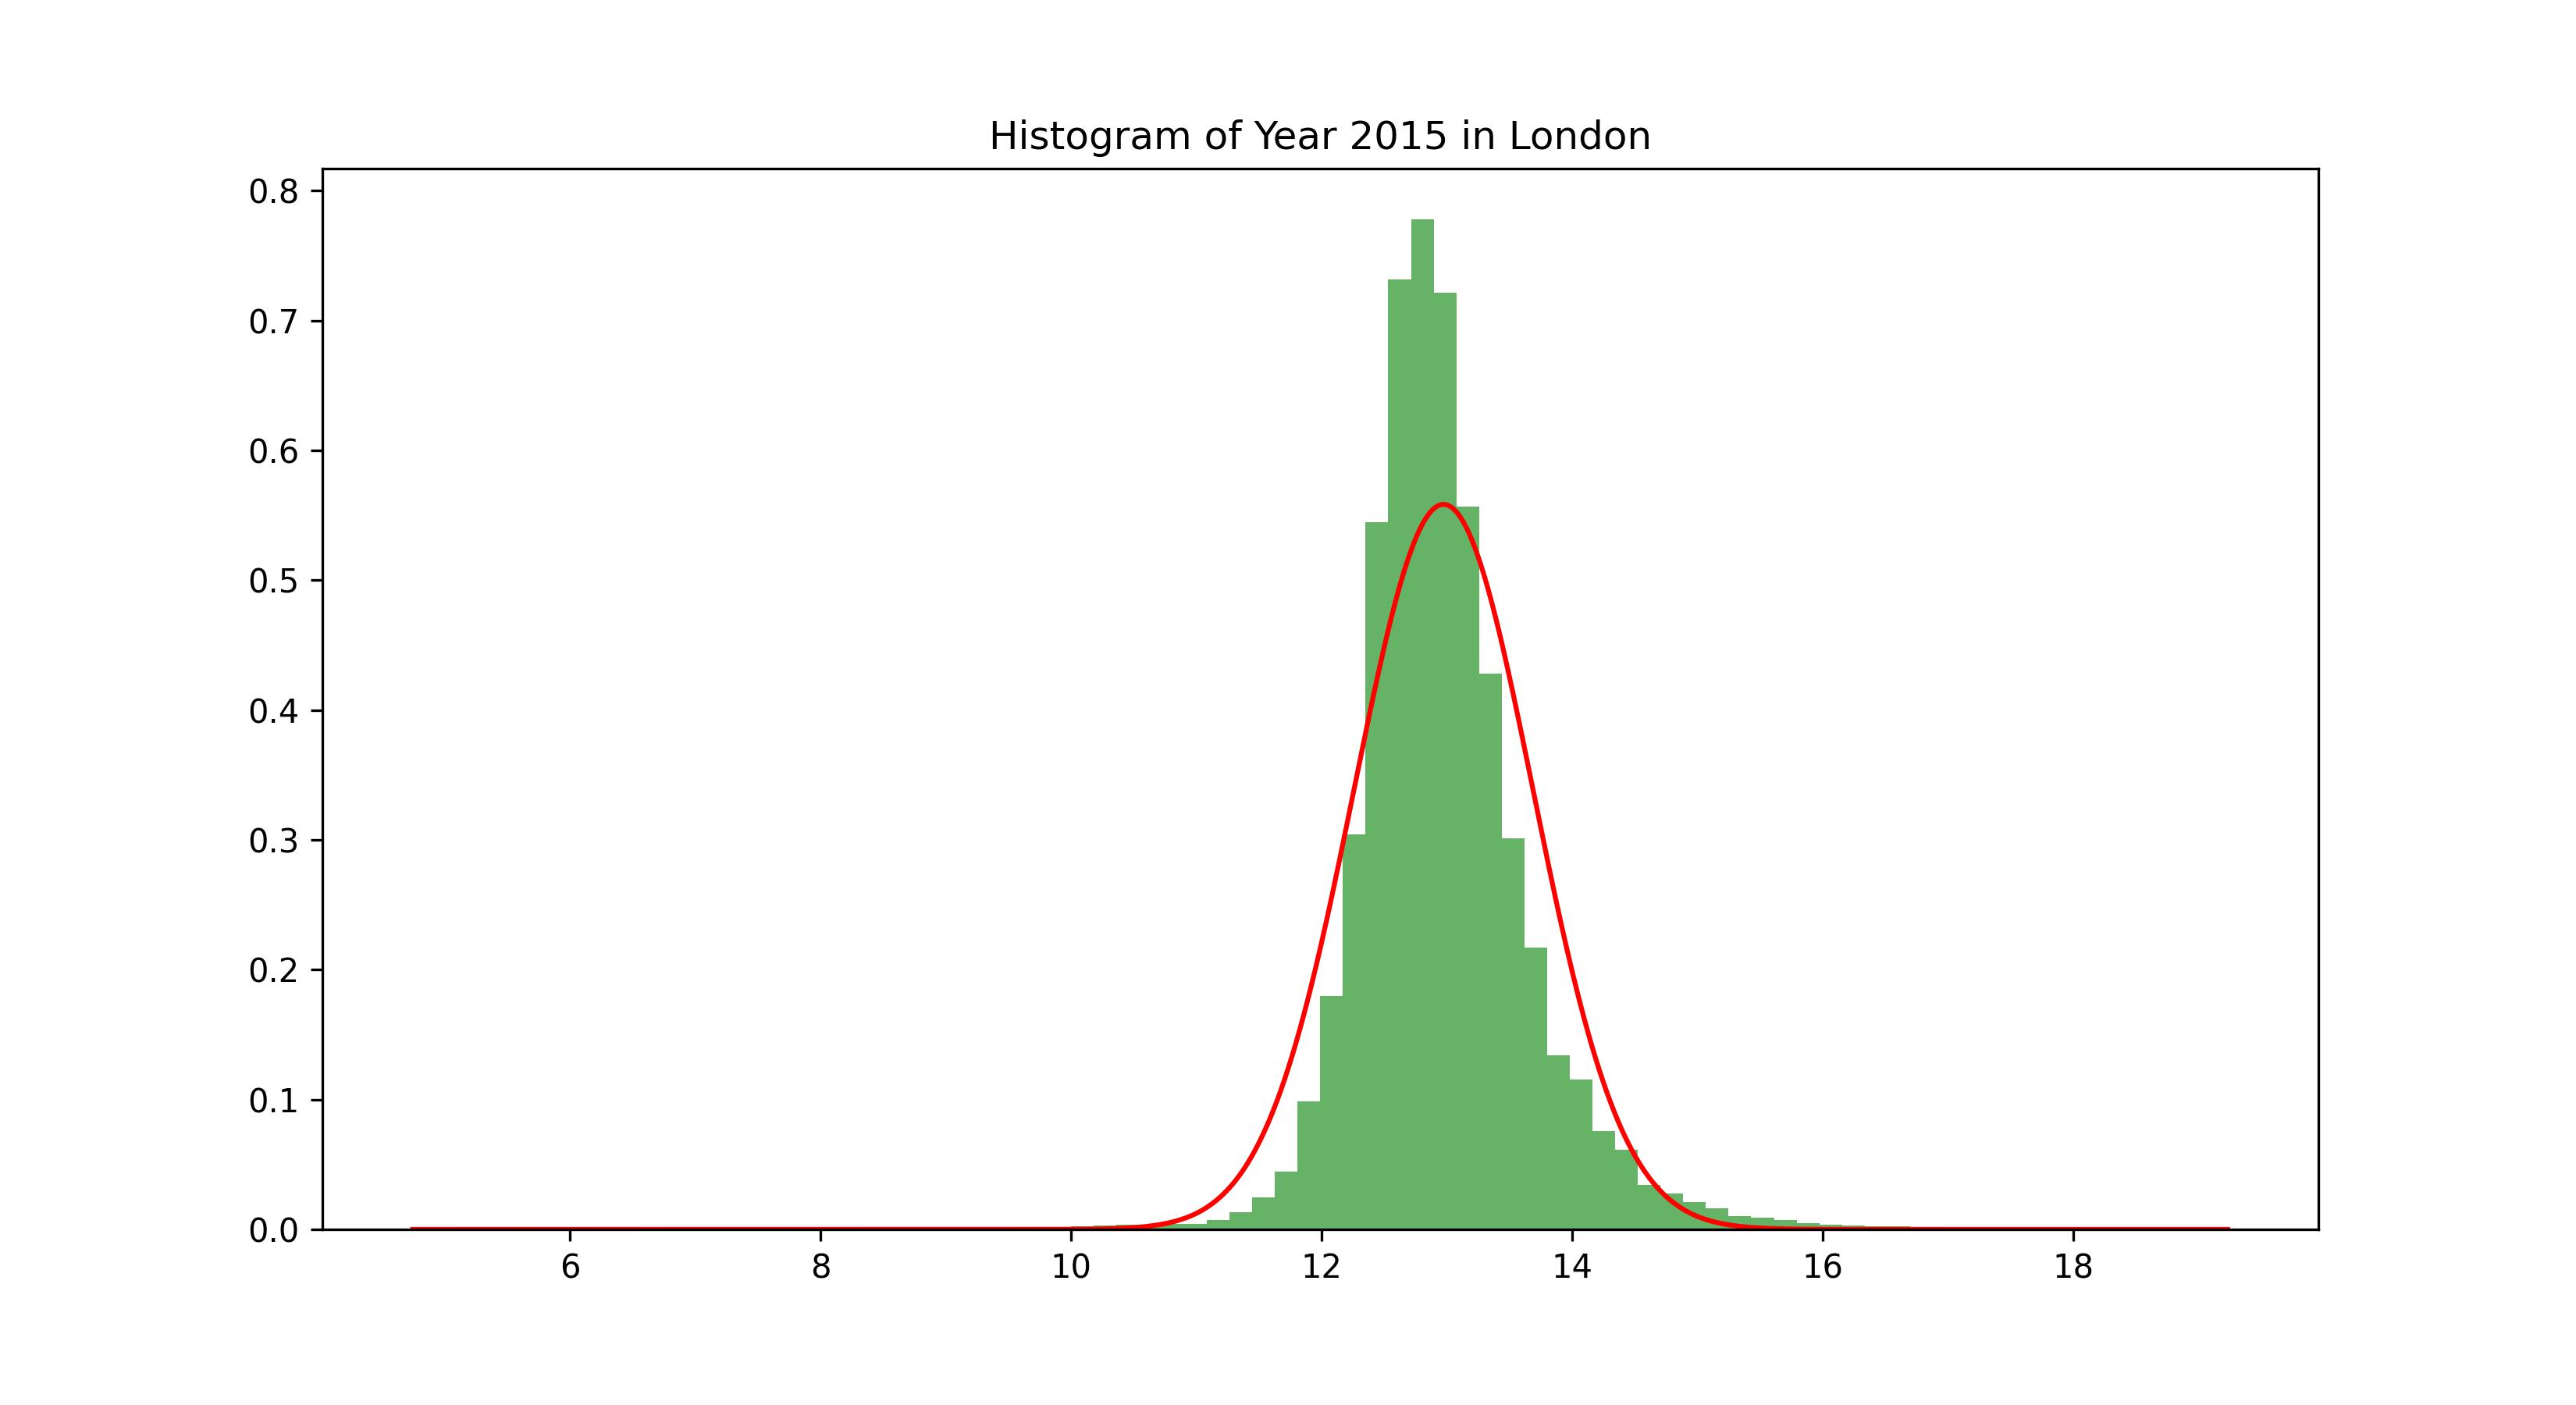
\includegraphics{compare_2015_London.jpg}
%     \caption{}\label{fig:qq}
% \end{figure}

\subsection{Region Definition}

We are only concerned with England in the UK and have split it into 9 regions. \
All research is based on these 9 regions. You can see this more closely in Figure (\ref{fig:ukmap})

\begin{figure}
    \centering
    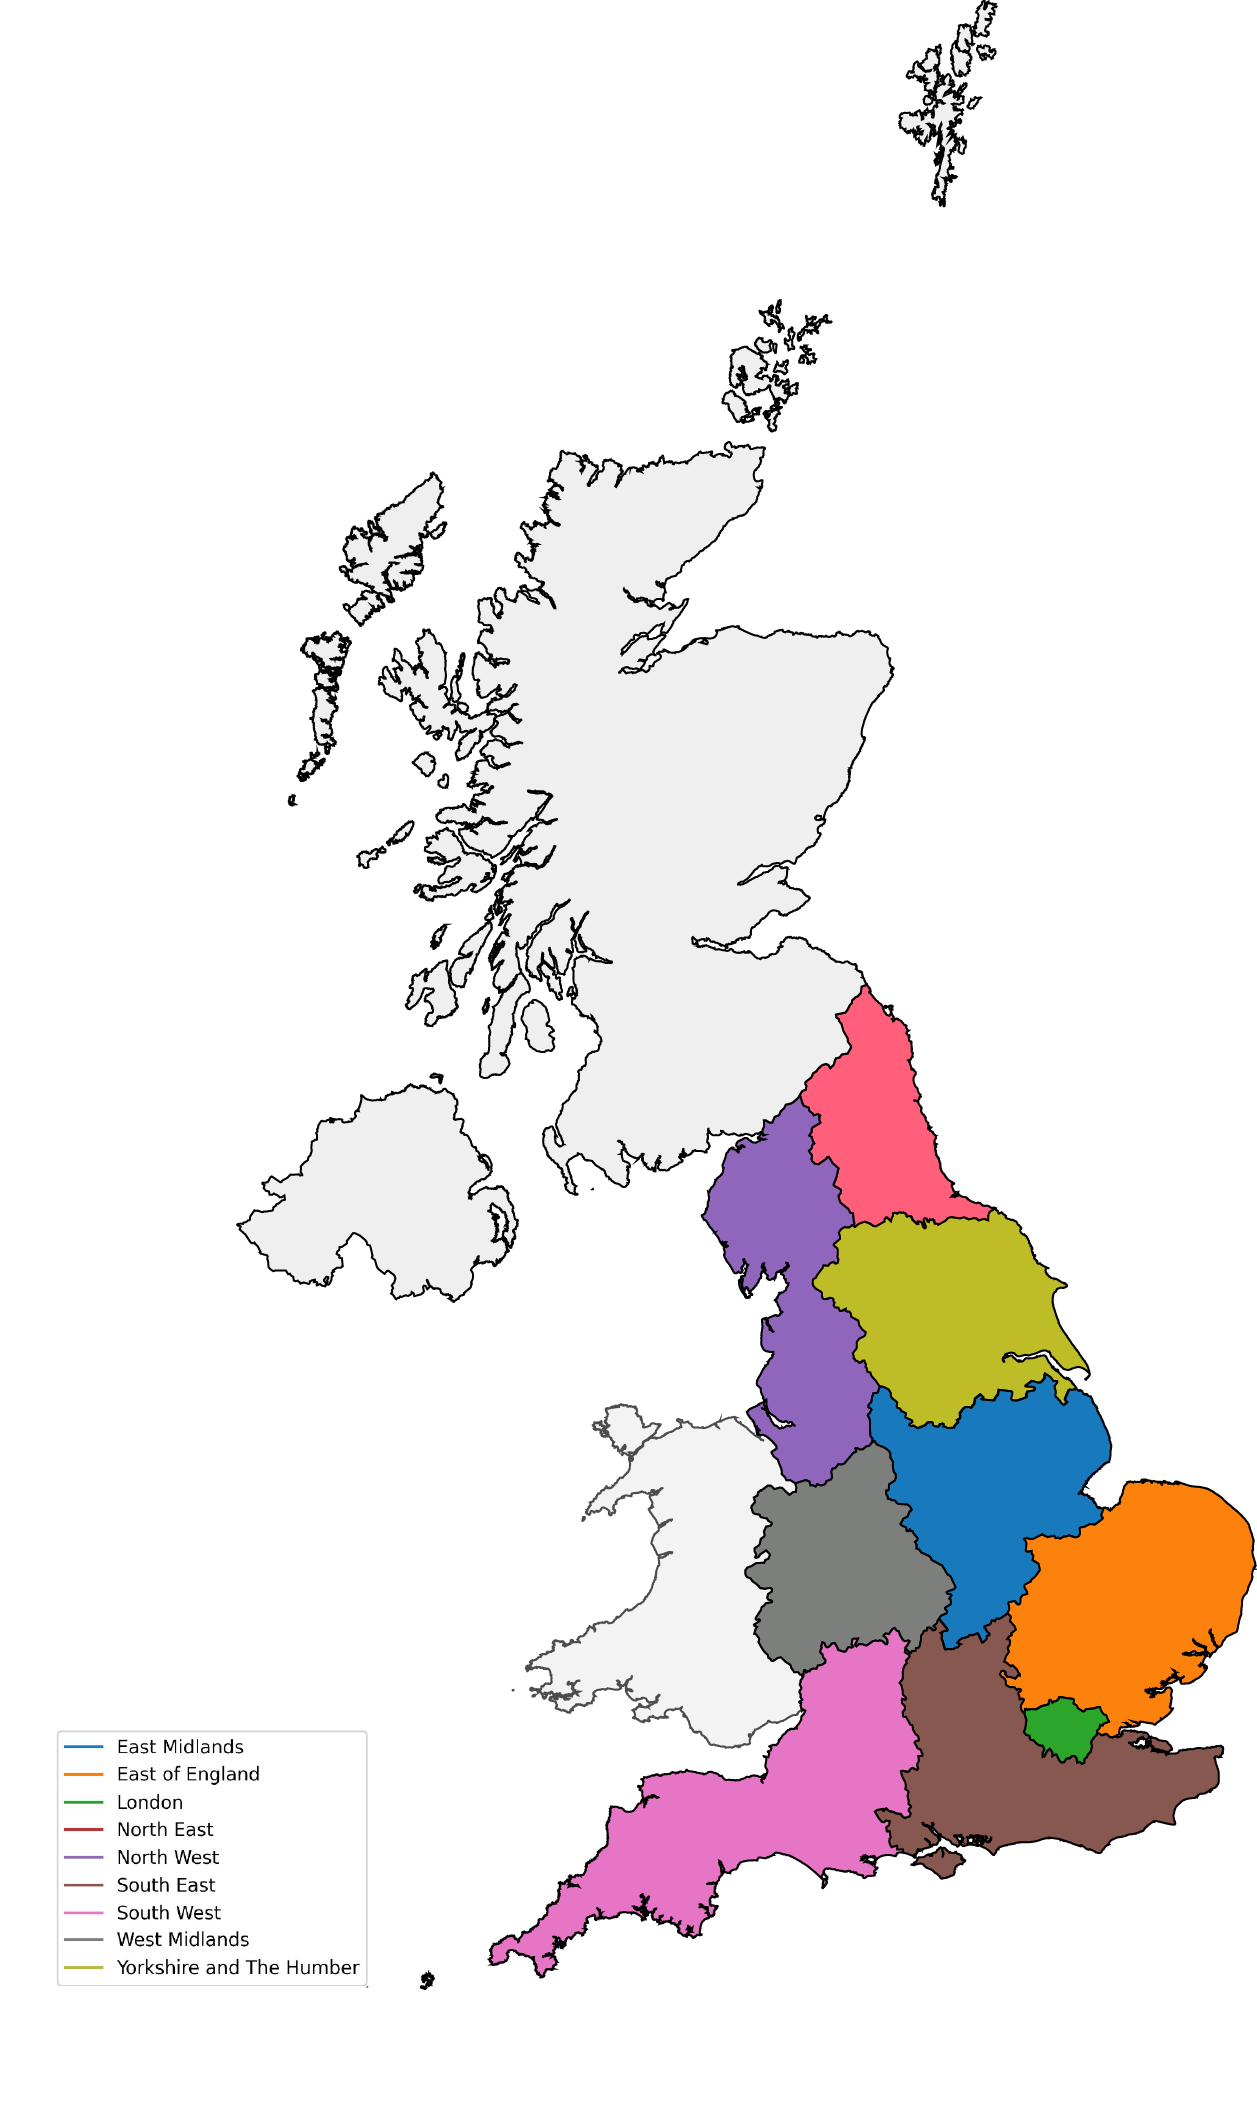
\includegraphics[width=.4\textwidth]{ukmap.png}
    \caption{The names of the regions and their corresponding colours are fixed later in the text, \
    i.e.: Blue for East Midlands, Orange for East of England, Green for London, Red for North East, \
    Purple for North West, Burnt Umber for South East, Lilac Pink for South West, Gray for West Midlands, \
    Yellow for Yorkshire and The Humber. Lilac Pink corresponds to the South West, Gray to the West Midlands, \
    and yellow to Yorkshire and The Humber. (Source: mapsvg.com \textsuperscript{\cite{map}})}\label{fig:ukmap}
\end{figure}


\section{The Models}
\subsection{Model of House Price}

\begin{figure}[htbp]
    \centering
    \begin{subfigure}[b]{.45\textwidth}
    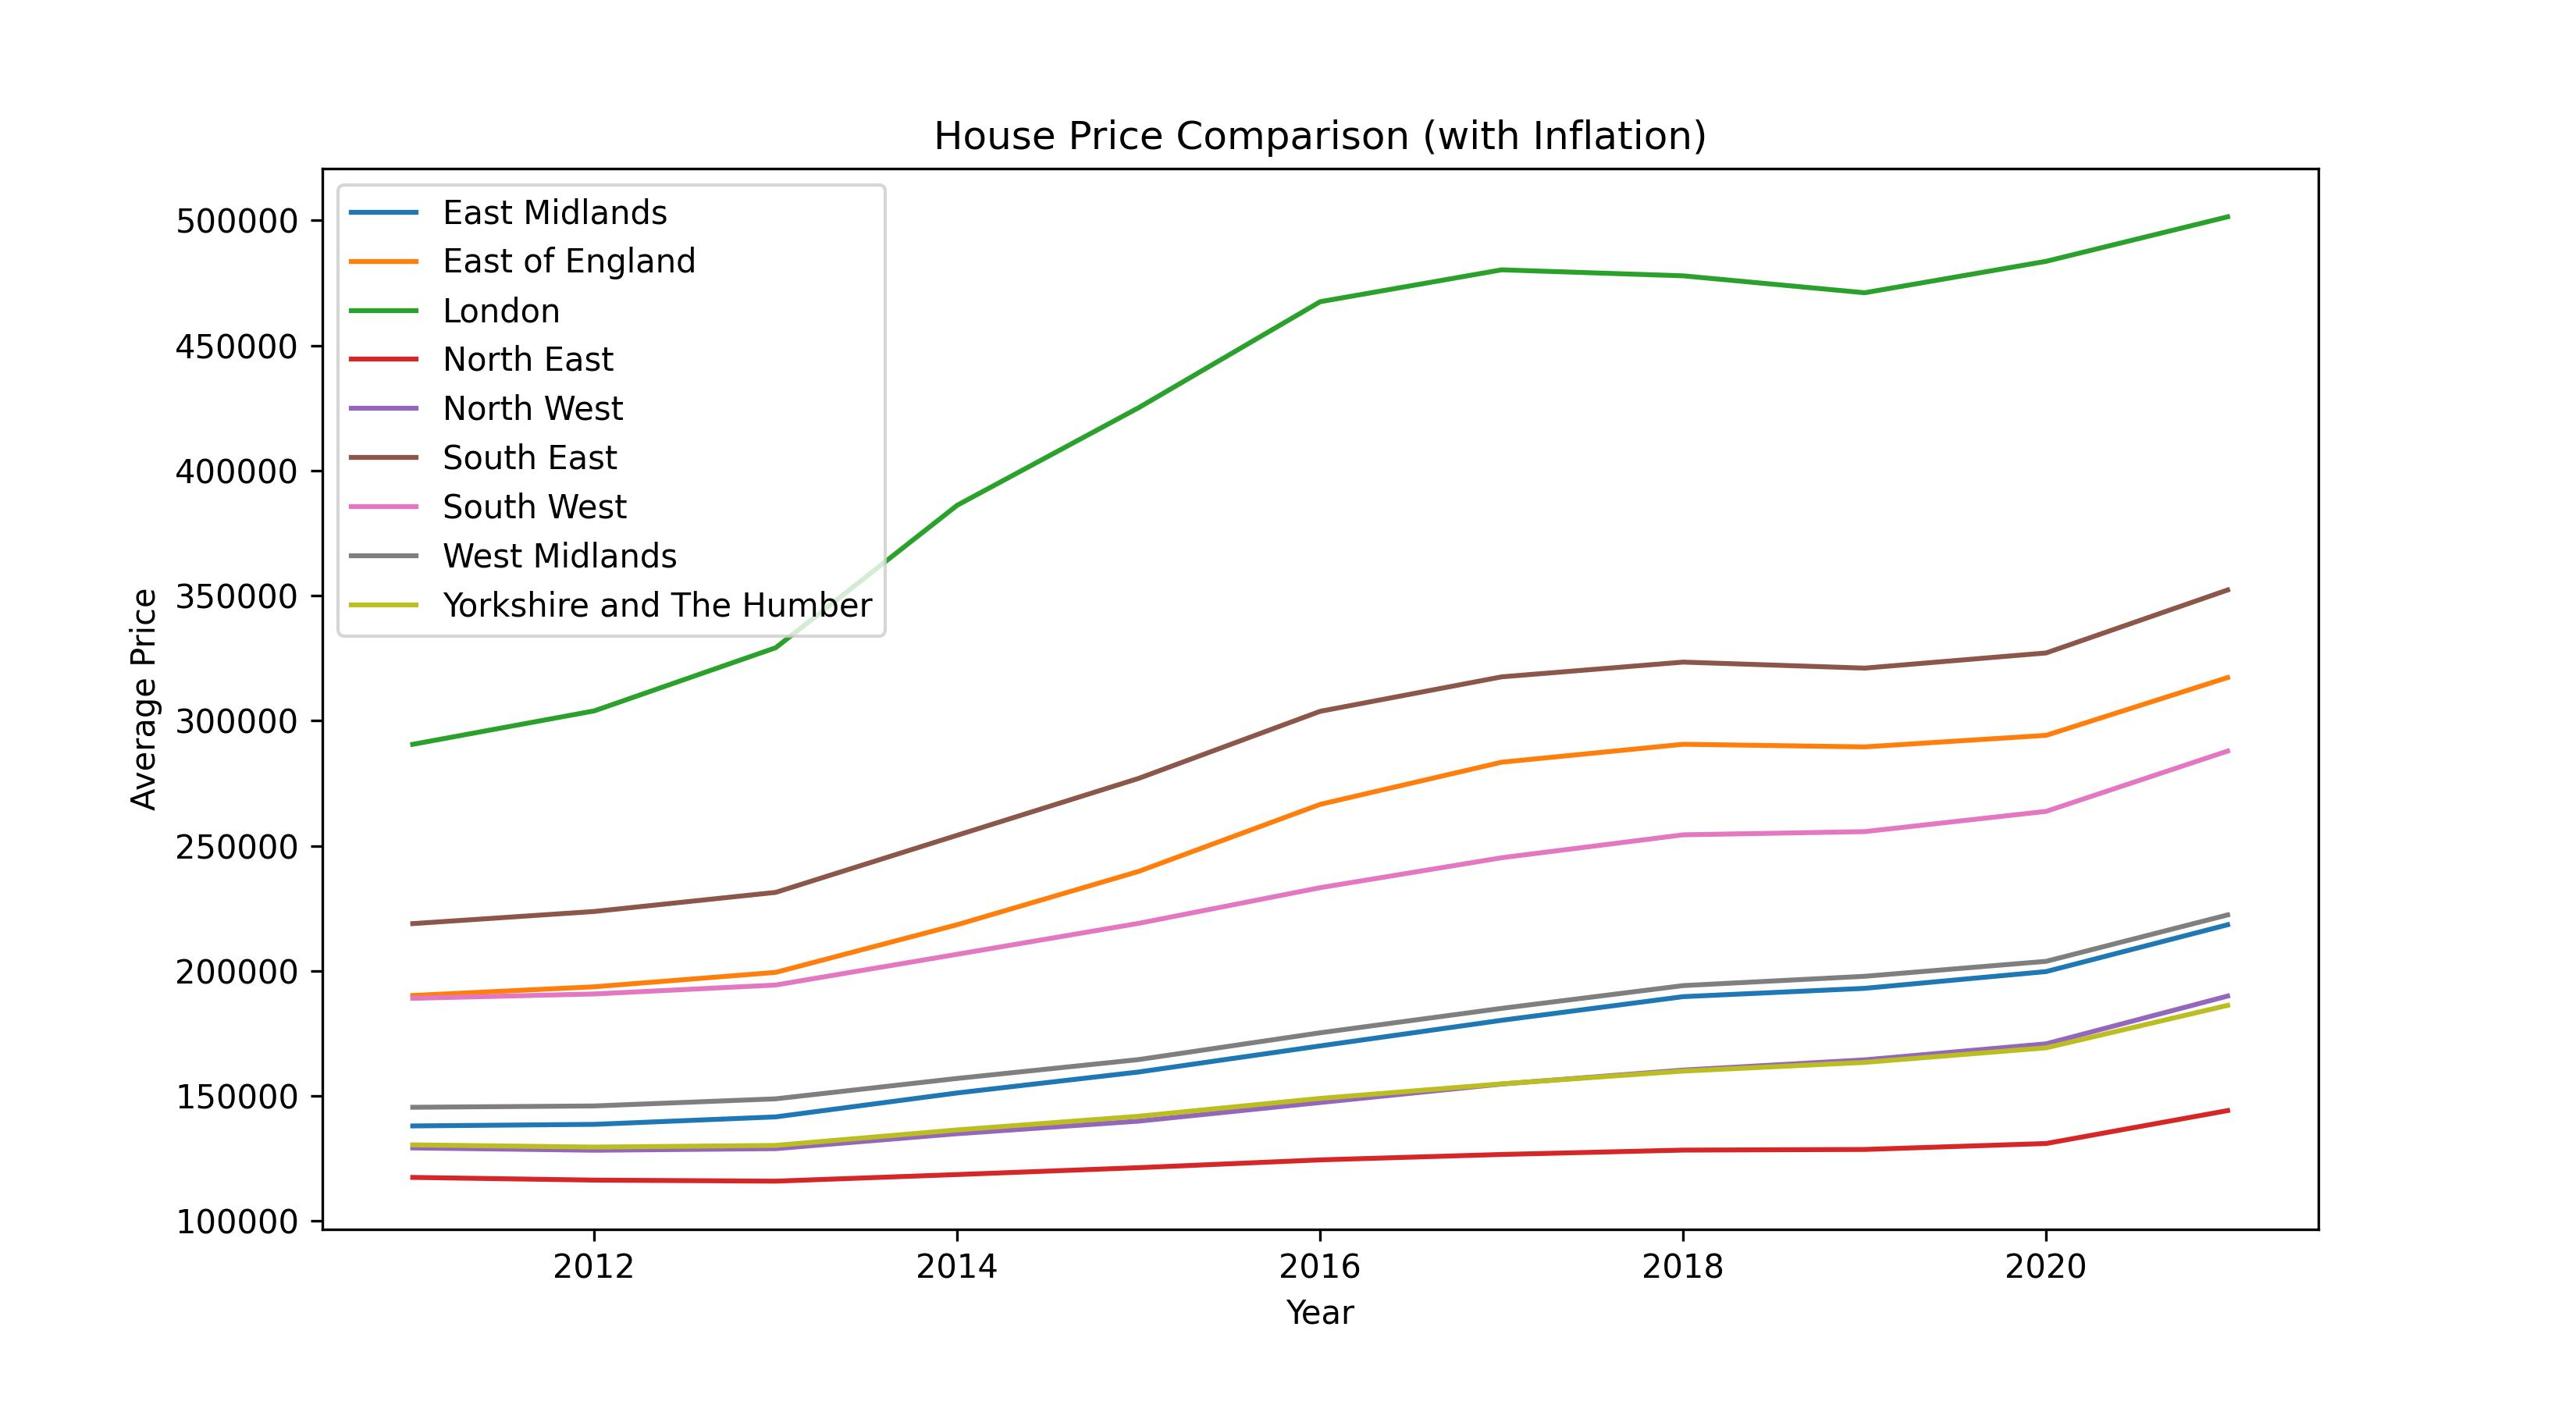
\includegraphics[width=\textwidth]{House Price Comparison (with Inflation).jpg}
    \caption{}\label{subfig:Inflation}
\end{subfigure}
\begin{subfigure}[b]{.45\textwidth}
    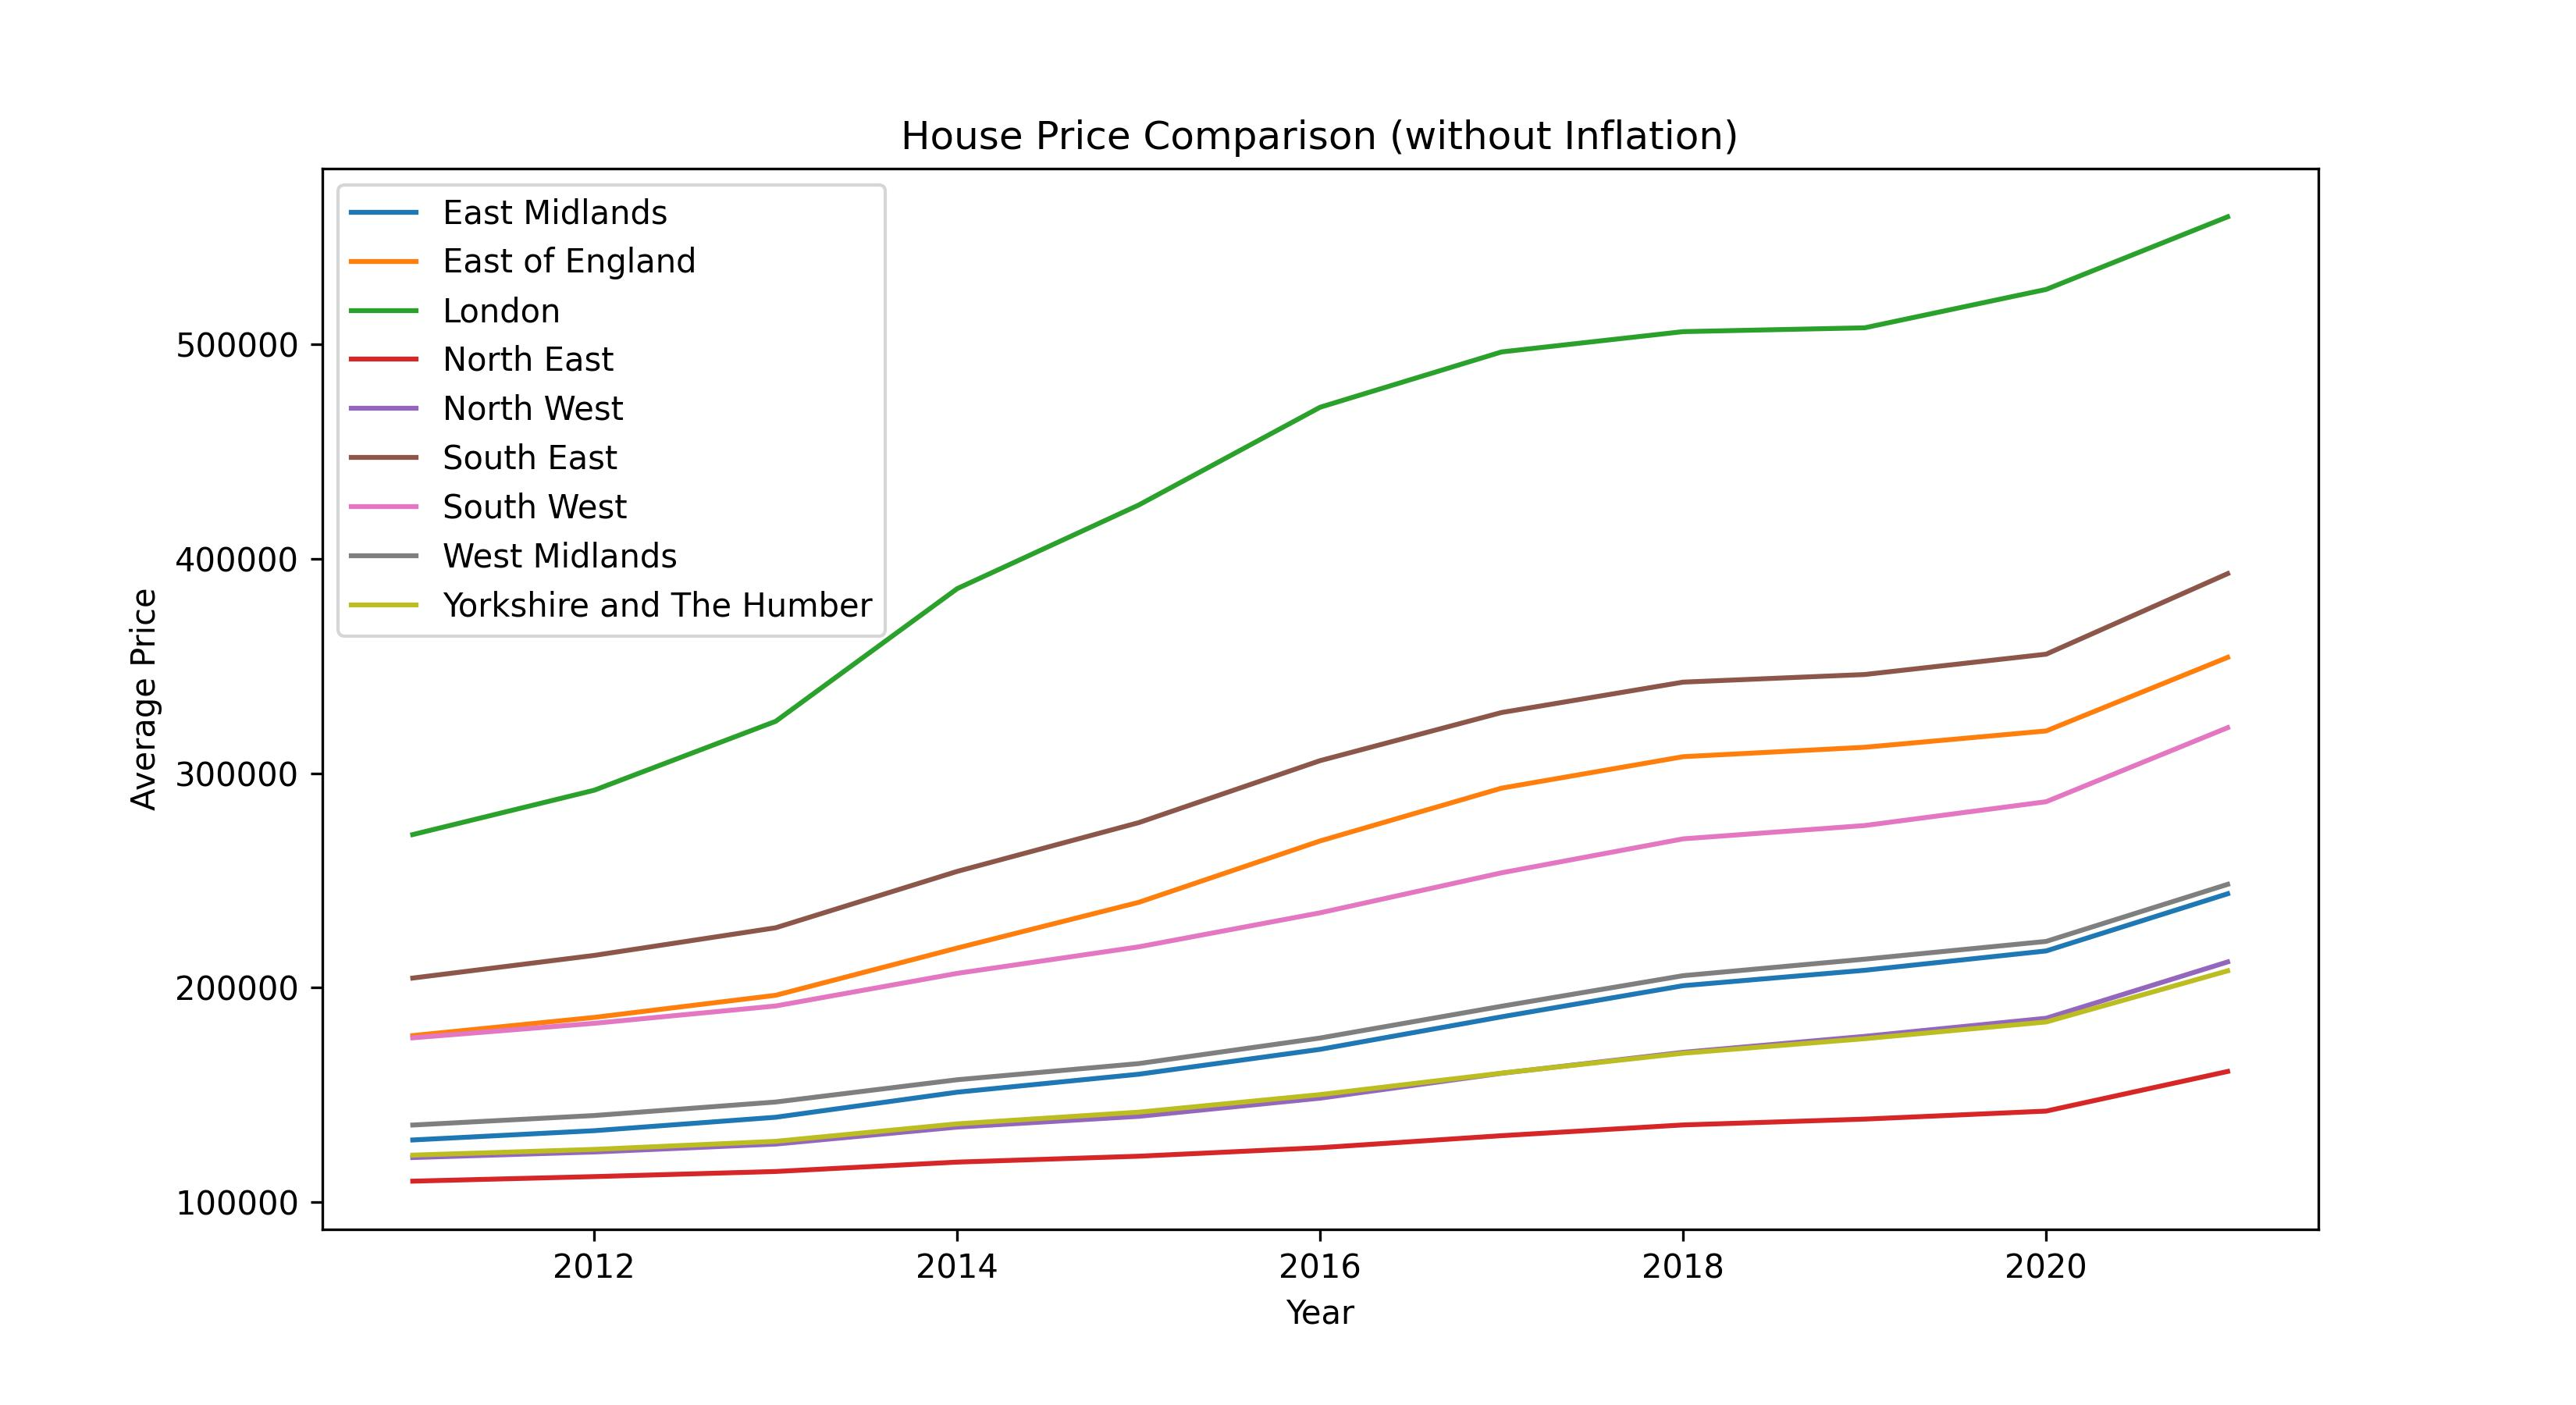
\includegraphics[width=\textwidth]{House Price Comparison (without Inflation).jpg}
    \caption{}\label{subfig:noInflation}
\end{subfigure}
\caption{Line chart (\ref{subfig:Inflation}) shows raw house price data for each UK \
region from 2011 to 2022, and line chart (\ref{subfig:noInflation}) shows inflation-adjusted\
house price data for each region.}\label{fig:houseprice}
\end{figure}
In this study, we first obtained annual house price data and data on each housing transaction within \
each year. It is important to note that we have chosen to use per transaction data rather than the \
summary data provided by the UK government, i.e. annual house price data. This is because the averages \
in the summary data are arithmetic averages and may not accurately reflect the true distribution of \
house prices. Instead, the per-transaction data provide a wealth of information that allows us to \
carry out a more detailed analysis of house prices, for example by considering the impact of factors \
such as regional differences on house prices. At the same time, we cannot ignore the impact of inflation. \
We therefore need to scale prices back to real house prices before fitting. \
These are illustrated in Figure (\ref{fig:houseprice})

Next, we log-transformed house prices to ensure that the distribution of house prices \
met the assumption of a normal distribution. This is because a normal distribution is \
a fundamental assumption in many statistical models, and satisfying it makes our model more robust.
\subsubsection{Result}
After fitting the price distributions for each year and region, we used a Q-Q plot \
(Quantile-Quantile Plot) to assess the accuracy of the model, which is a graphical \
tool to test whether two probability distributions are similar by comparing their quartiles, \
and from Figure (\ref{fig:qq}) we can see that the points on the Q-Q plot fall roughly on a straight line.

\begin{figure}[htbp]
    \centering
    \begin{subfigure}[b]{.5\textwidth}
        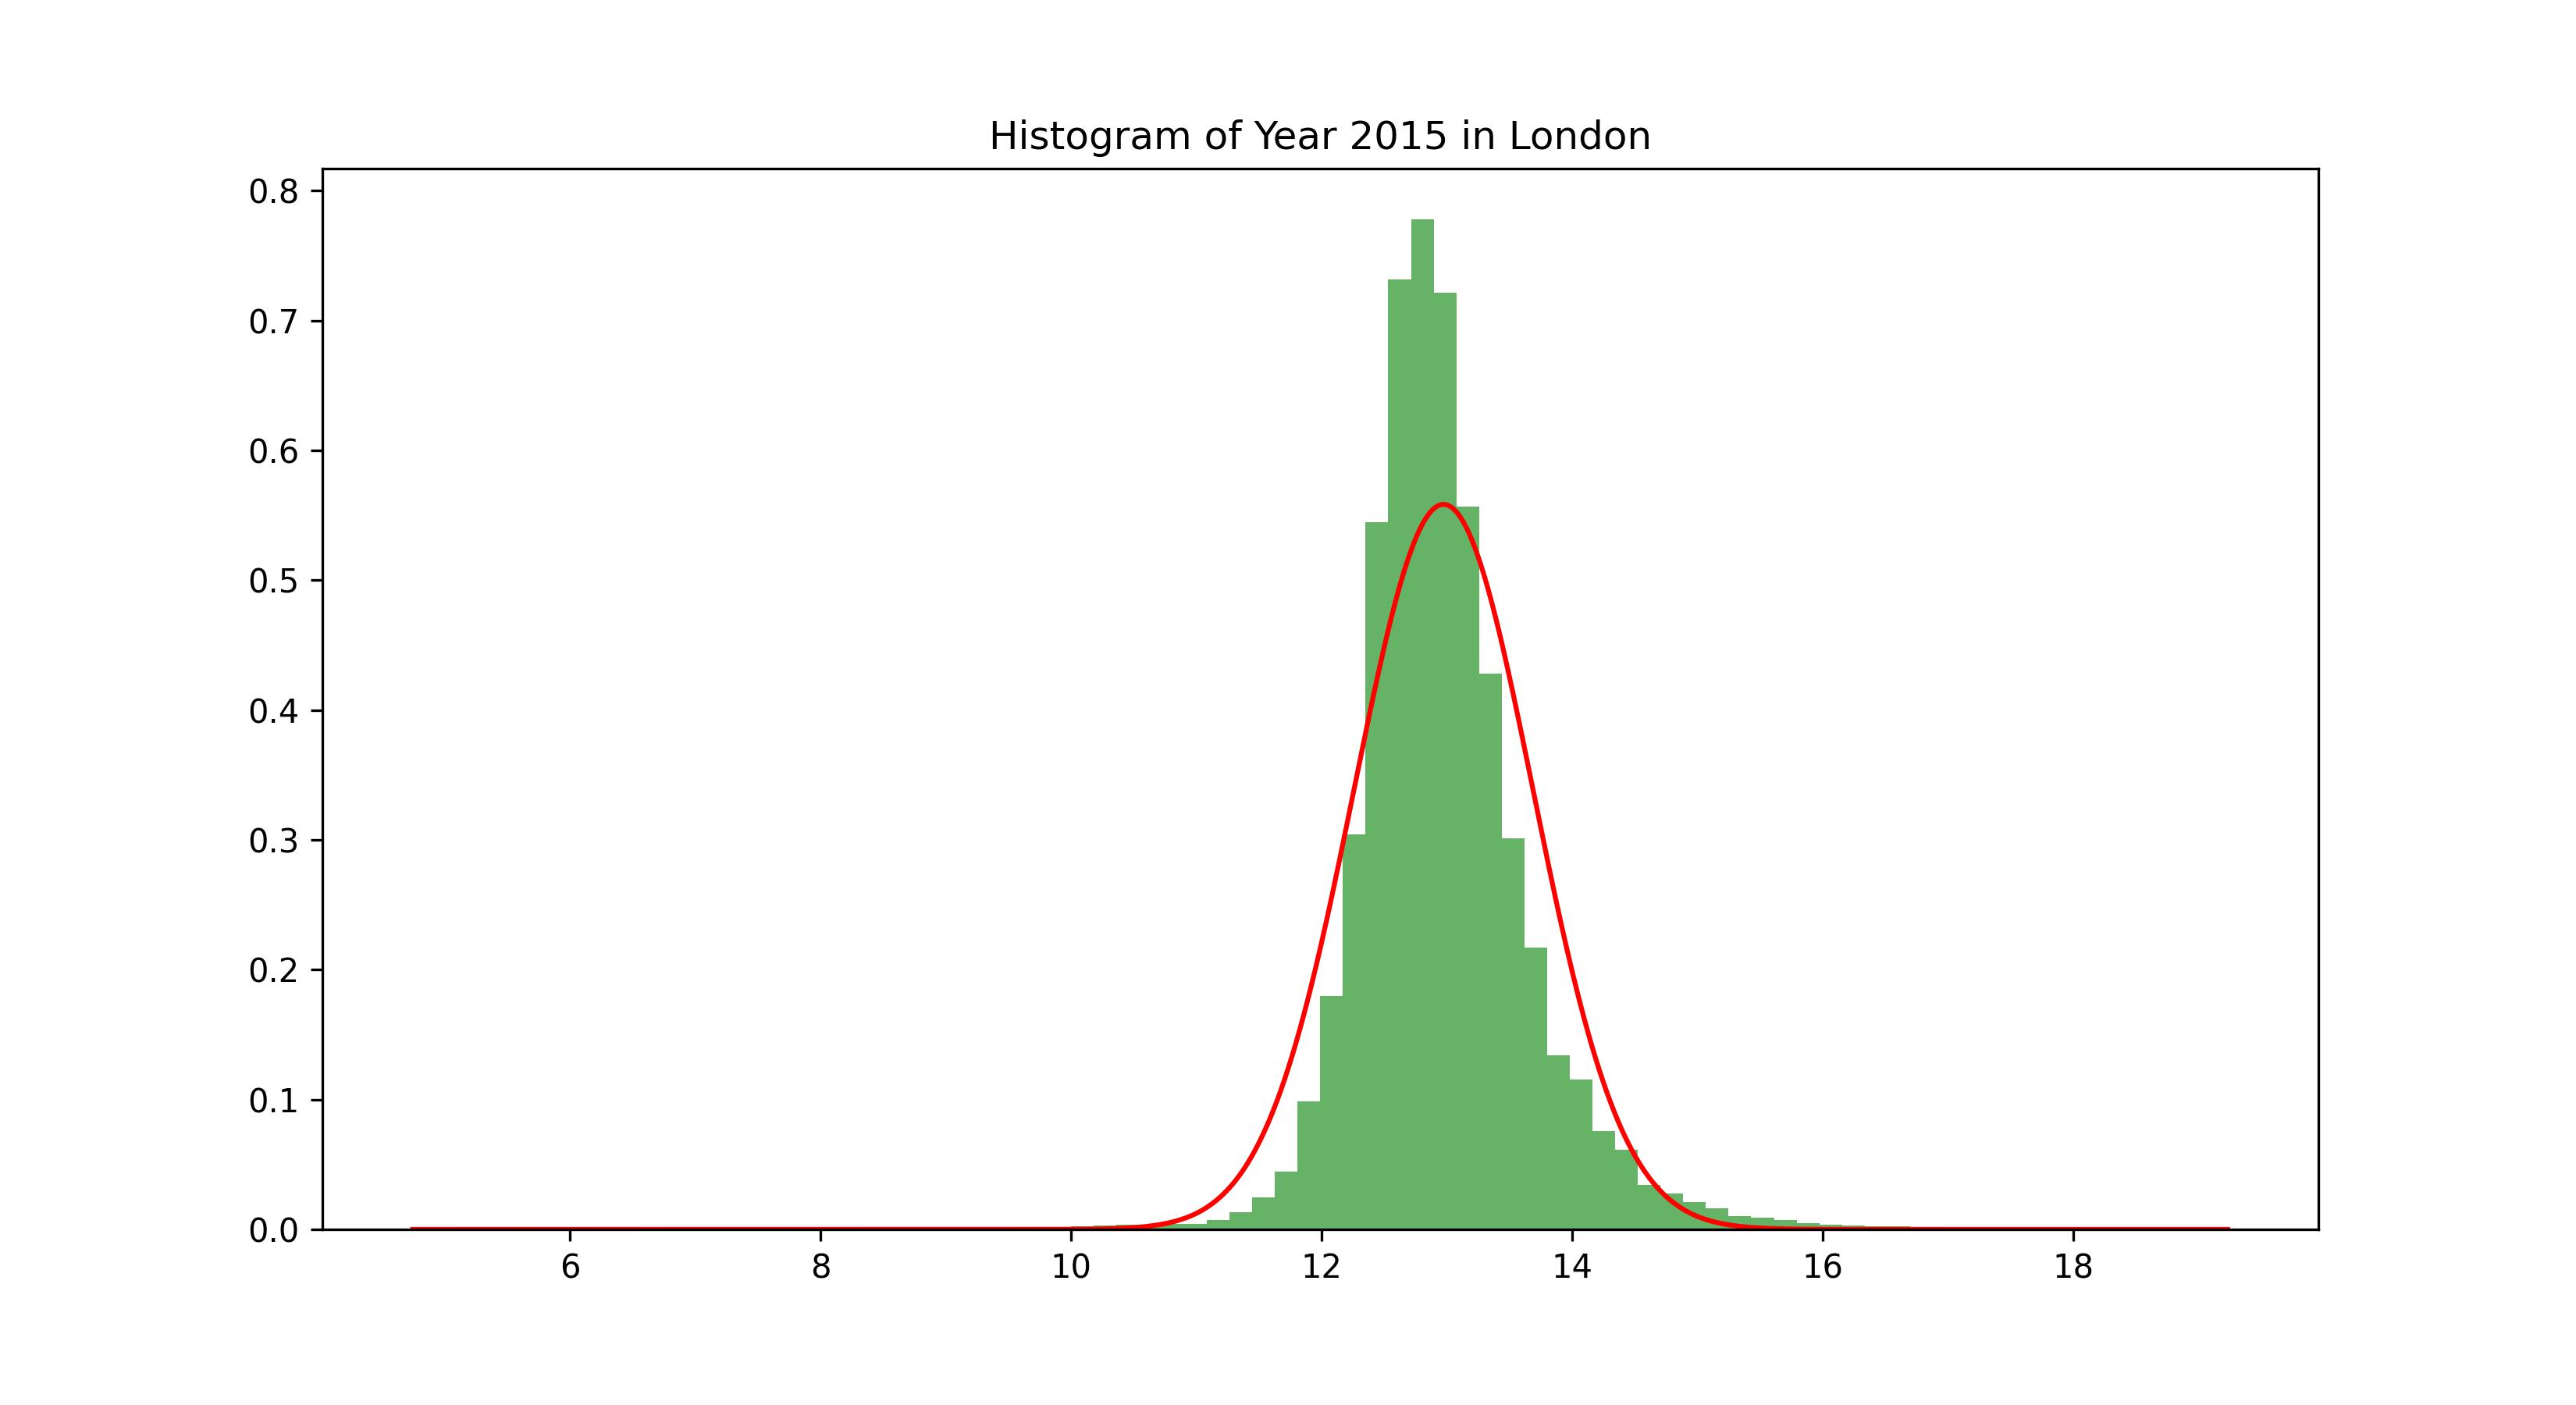
\includegraphics[width=\textwidth]{compare_2015_London.jpg}
        \caption{}\label{subfig:hist}
    \end{subfigure}
    \begin{subfigure}[b]{.4\textwidth}
        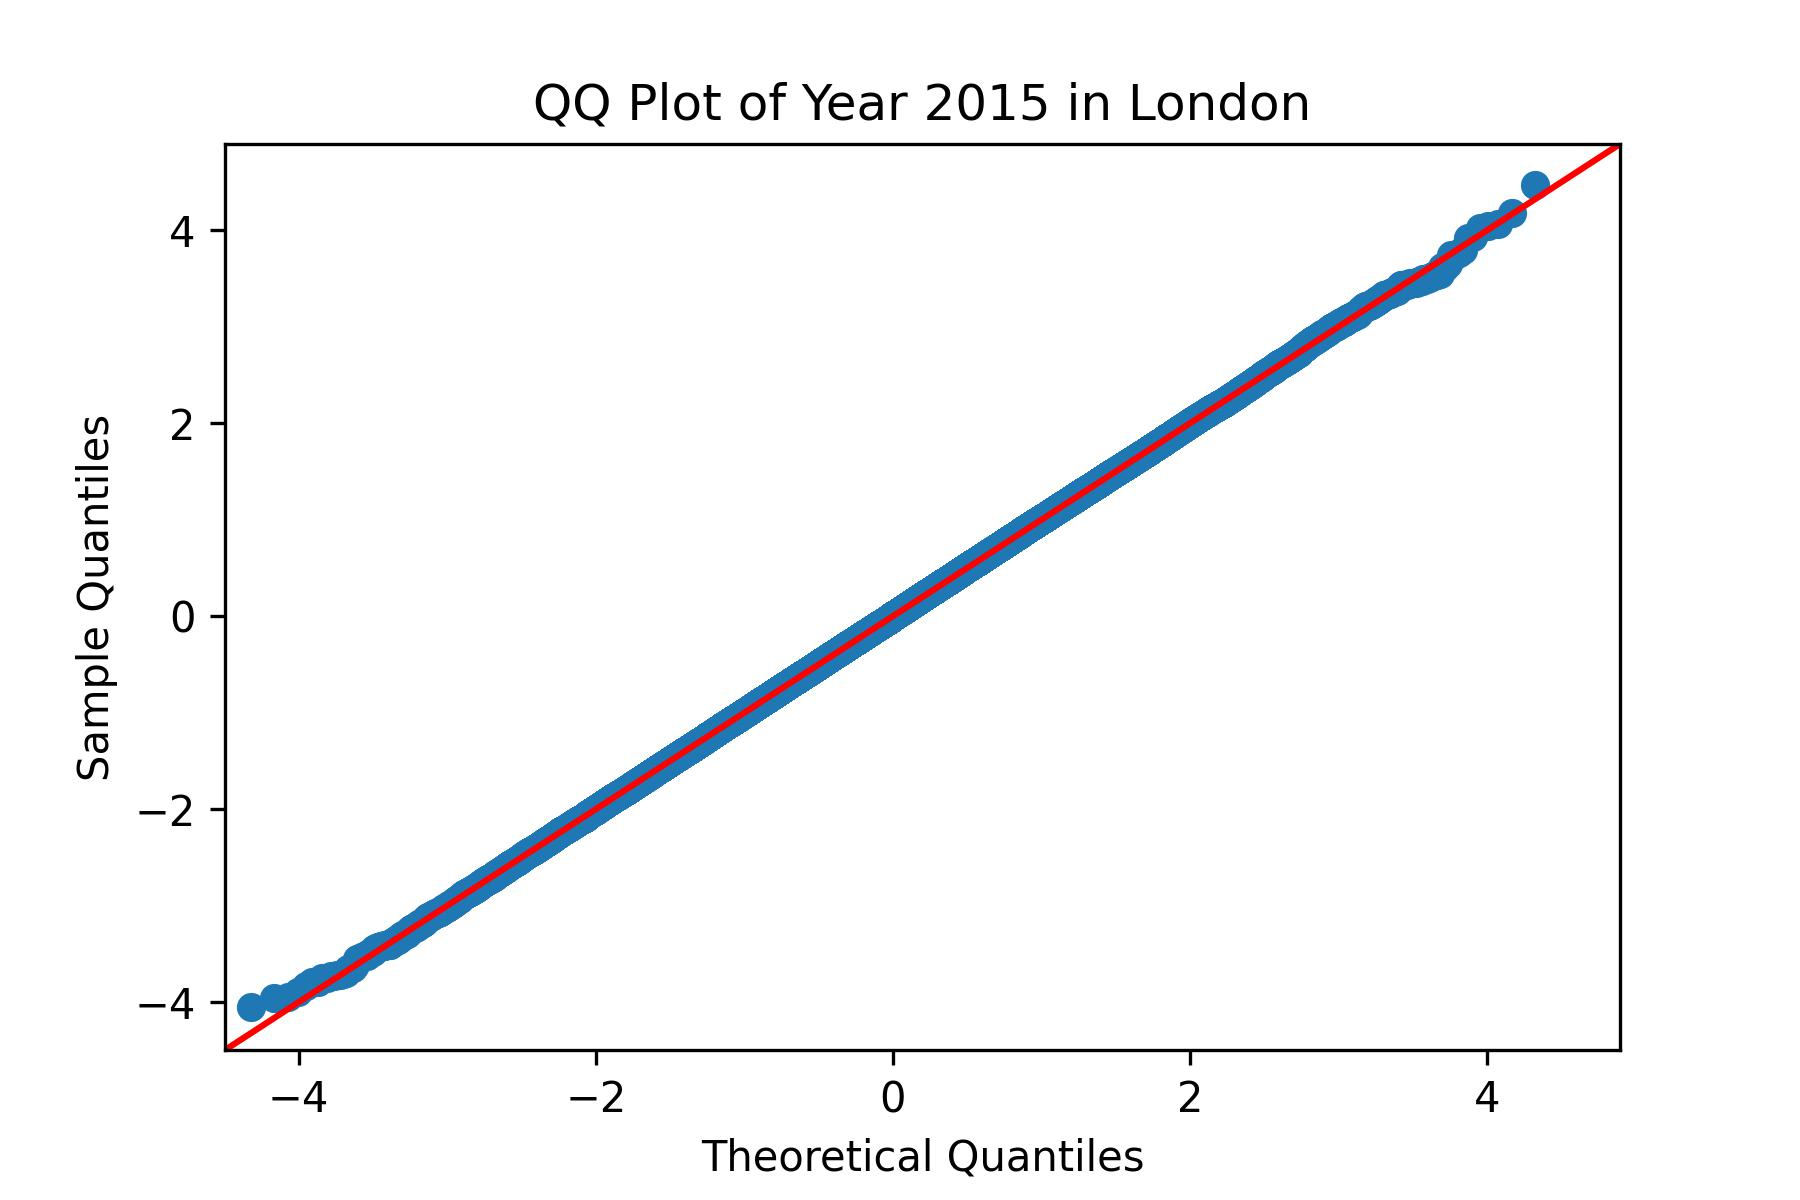
\includegraphics[width=\textwidth]{qq_2015_London.jpg}
        \caption{}\label{subfig:qq}
    \end{subfigure}
    \caption{Only the logarithmically fitted house price data for London in 2015 are shown here, i.e. Figure (\ref{subfig:hist})\
    and the Q-Q plot (\ref{subfig:qq}). You can see that the prices fit well around the\
    mean, but there are some deviations around the very large and very small values.
    }\label{fig:qq}
\end{figure}

\subsubsection{Details about Model of House Price}
We start with the assumption that house prices, when adjusted for inflation ($A_i$), are normally distributed. A normal distribution is parameterized by its mean ($\mu$) and variance ($\sigma^2$), and its probability density function (pdf) is given by:

\begin{equation}
f(x|\mu, \sigma^2)=\frac{1}{\sqrt{2\pi\sigma^2}} e^{-\frac{(x-\mu)^2}{2\sigma^2}}
\end{equation}

Given this, the likelihood function $L(\mu, \sigma^2|x)$ for observing a particular house price $x$ is equal to the pdf of that house price, given the parameters:

\begin{equation}
L(\mu, \sigma^2|x)=f(x|\mu, \sigma^2)
\end{equation}

If we have observed a set of house prices $X={x_1, x_2, ..., x_n}$, we can construct the joint likelihood function for the entire dataset as the product of the individual likelihoods, because we assume the observations are independent:

\begin{equation}
L(\mu, \sigma^2|X)=\prod_{i=1}^{n} f(x_i|\mu, \sigma^2)
\end{equation}

The MLE estimates for $\mu$ and $\sigma^2$ are the values that maximize this likelihood function.

Now, it's much easier to work with the log of the likelihood function, known as the log-likelihood. This is because the log-likelihood turns our product into a sum, which is computationally simpler:

\begin{equation}
\log L(\mu, \sigma^2|X)=\sum_{i=1}^{n} \log f(x_i|\mu, \sigma^2)
\end{equation}

Taking the derivative of the log-likelihood with respect to $\mu$ and $\sigma^2$, setting these derivatives equal to zero, and solving for $\mu$ and $\sigma^2$ gives the MLEs. This procedure results in the following MLEs:

\begin{equation}
\hat{\mu}=E[A_i]
\end{equation}

\begin{equation}
\hat{\sigma^2}=Var[A_i]
\end{equation}

Where $\hat{\mu}$ is the sample mean of house prices adjusted for inflation, and $\hat{\sigma^2}$ is the sample variance. These estimates maximize the likelihood of observing the data given the specified model. This approach is based on the statistical theory and the properties of the normal distribution.\\
This formula shows that $a_i$ (i.e. house price excluding inflation) is determined by a combination of $A_i$ (i.e. house price in the presence of inflation) and CPI (i.e. consumer price index), where CPI[year]/CPI[2015] is an adjustment factor to remove the effect of inflation. Here we have the same assumptions as the UK government and set 2015 as the base year.
\textsuperscript{\cite{guide}} \


\subsection{Model of the Number of Fires Per Year}
\subsubsection{Conclusion of the Model}
For the fire occurrence model, we first obtained detailed information on the number of 
fires that occurred in each area on each day, including the area where the fire 
occurred, the cause of the fire and the type of fire. This provided us with a wealth 
of information that allowed us to carry out a detailed analysis of the number of fires.

We then counted the number of residential fires per year and the total number of fires 
per year separately. We used a great likelihood estimation method to estimate the exponential 
distribution of the number of fires for these two types of fires. The exponential distribution 
is a commonly used probability distribution that describes the interval between events 
and is suitable for describing the time interval between the occurrence of independent 
random events. Great likelihood estimation allows us to obtain the most likely exponential 
distribution describing the number of fires.

We then used Monte Carlo simulation methods to obtain the probability distribution of 
each fire occurring in a dwelling. Monte Carlo simulation is a method of calculating 
the numerical solution of a physical quantity by repeated random sampling and can 
help us to better understand and predict the probability of fire occurrence.

Finally, we obtain a distribution of the total number of fires, $N$. 
This distribution describes the number of fires that occur in a given 
period of time and gives us important information about the frequency of fires.

Overall, our fire number model is as accurate and robust as possible through 
the use of detailed fire data, large probability estimation and Monte Carlo simulation.

\begin{figure}[htbp]
\centering
\begin{subfigure}[b]{.45\textwidth}
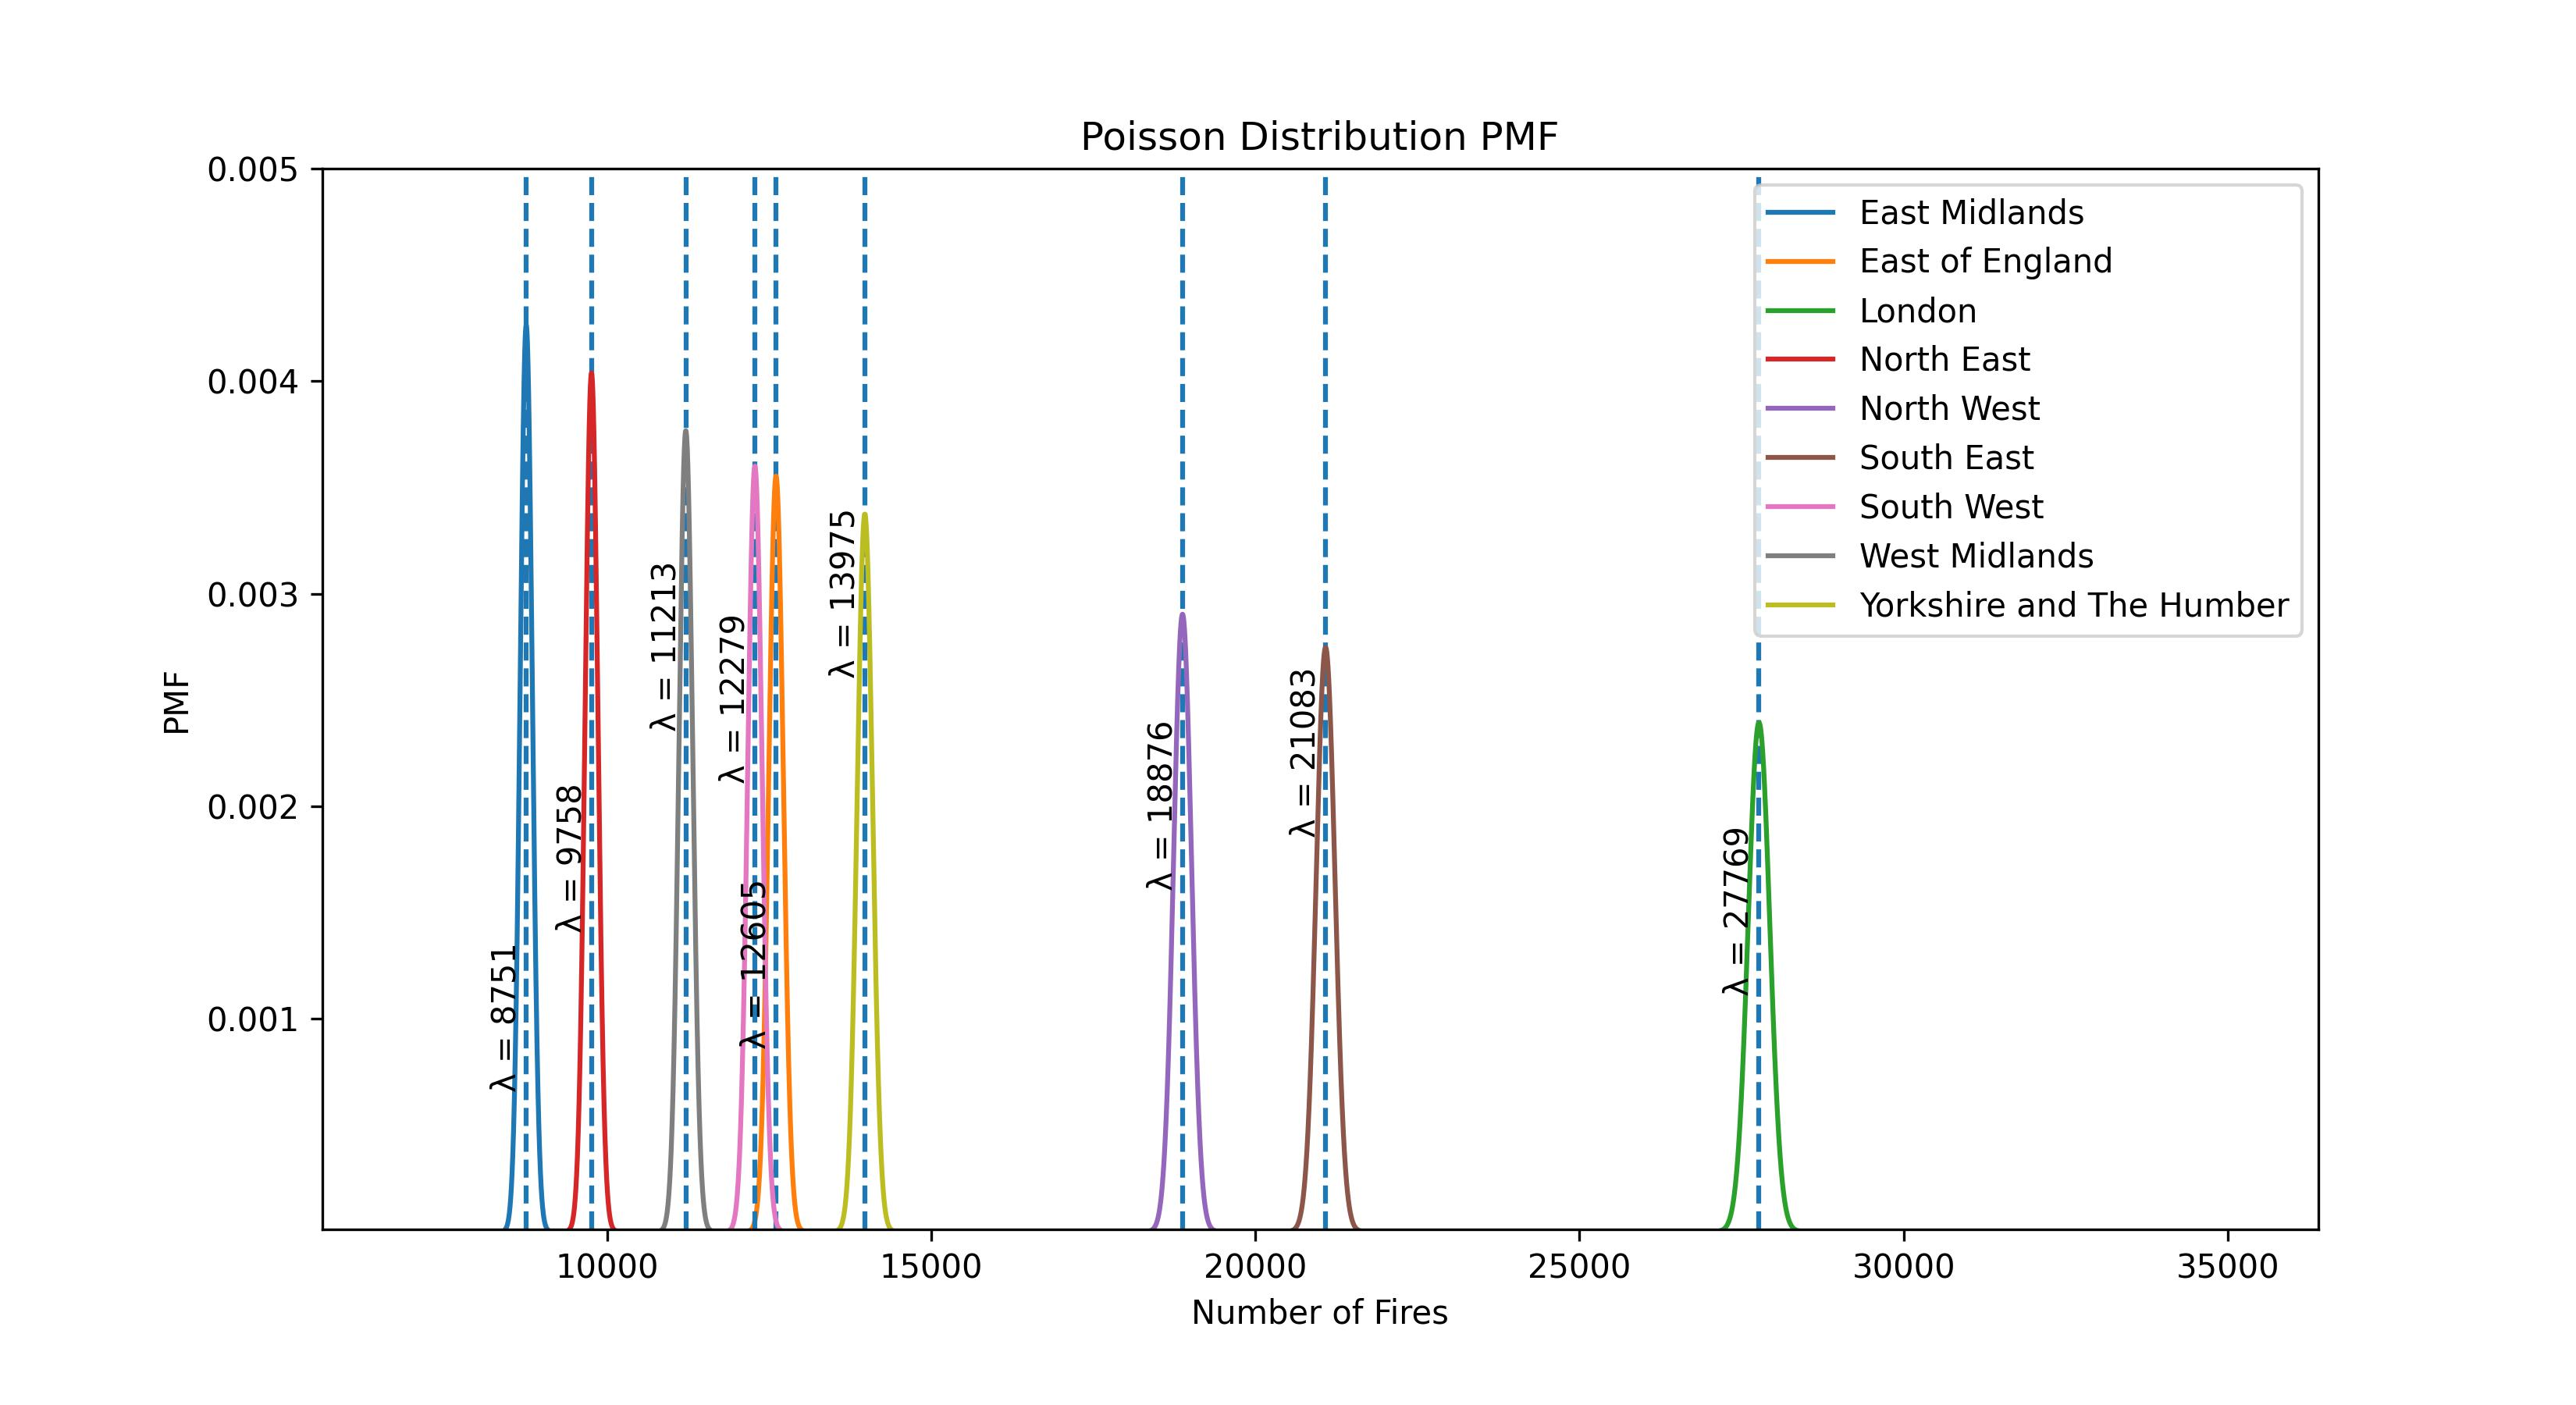
\includegraphics[width=\textwidth]{fire_times_pmf.jpg}
\caption{}\label{subfig:fireall}
\end{subfigure}
\begin{subfigure}[b]{.45\textwidth}
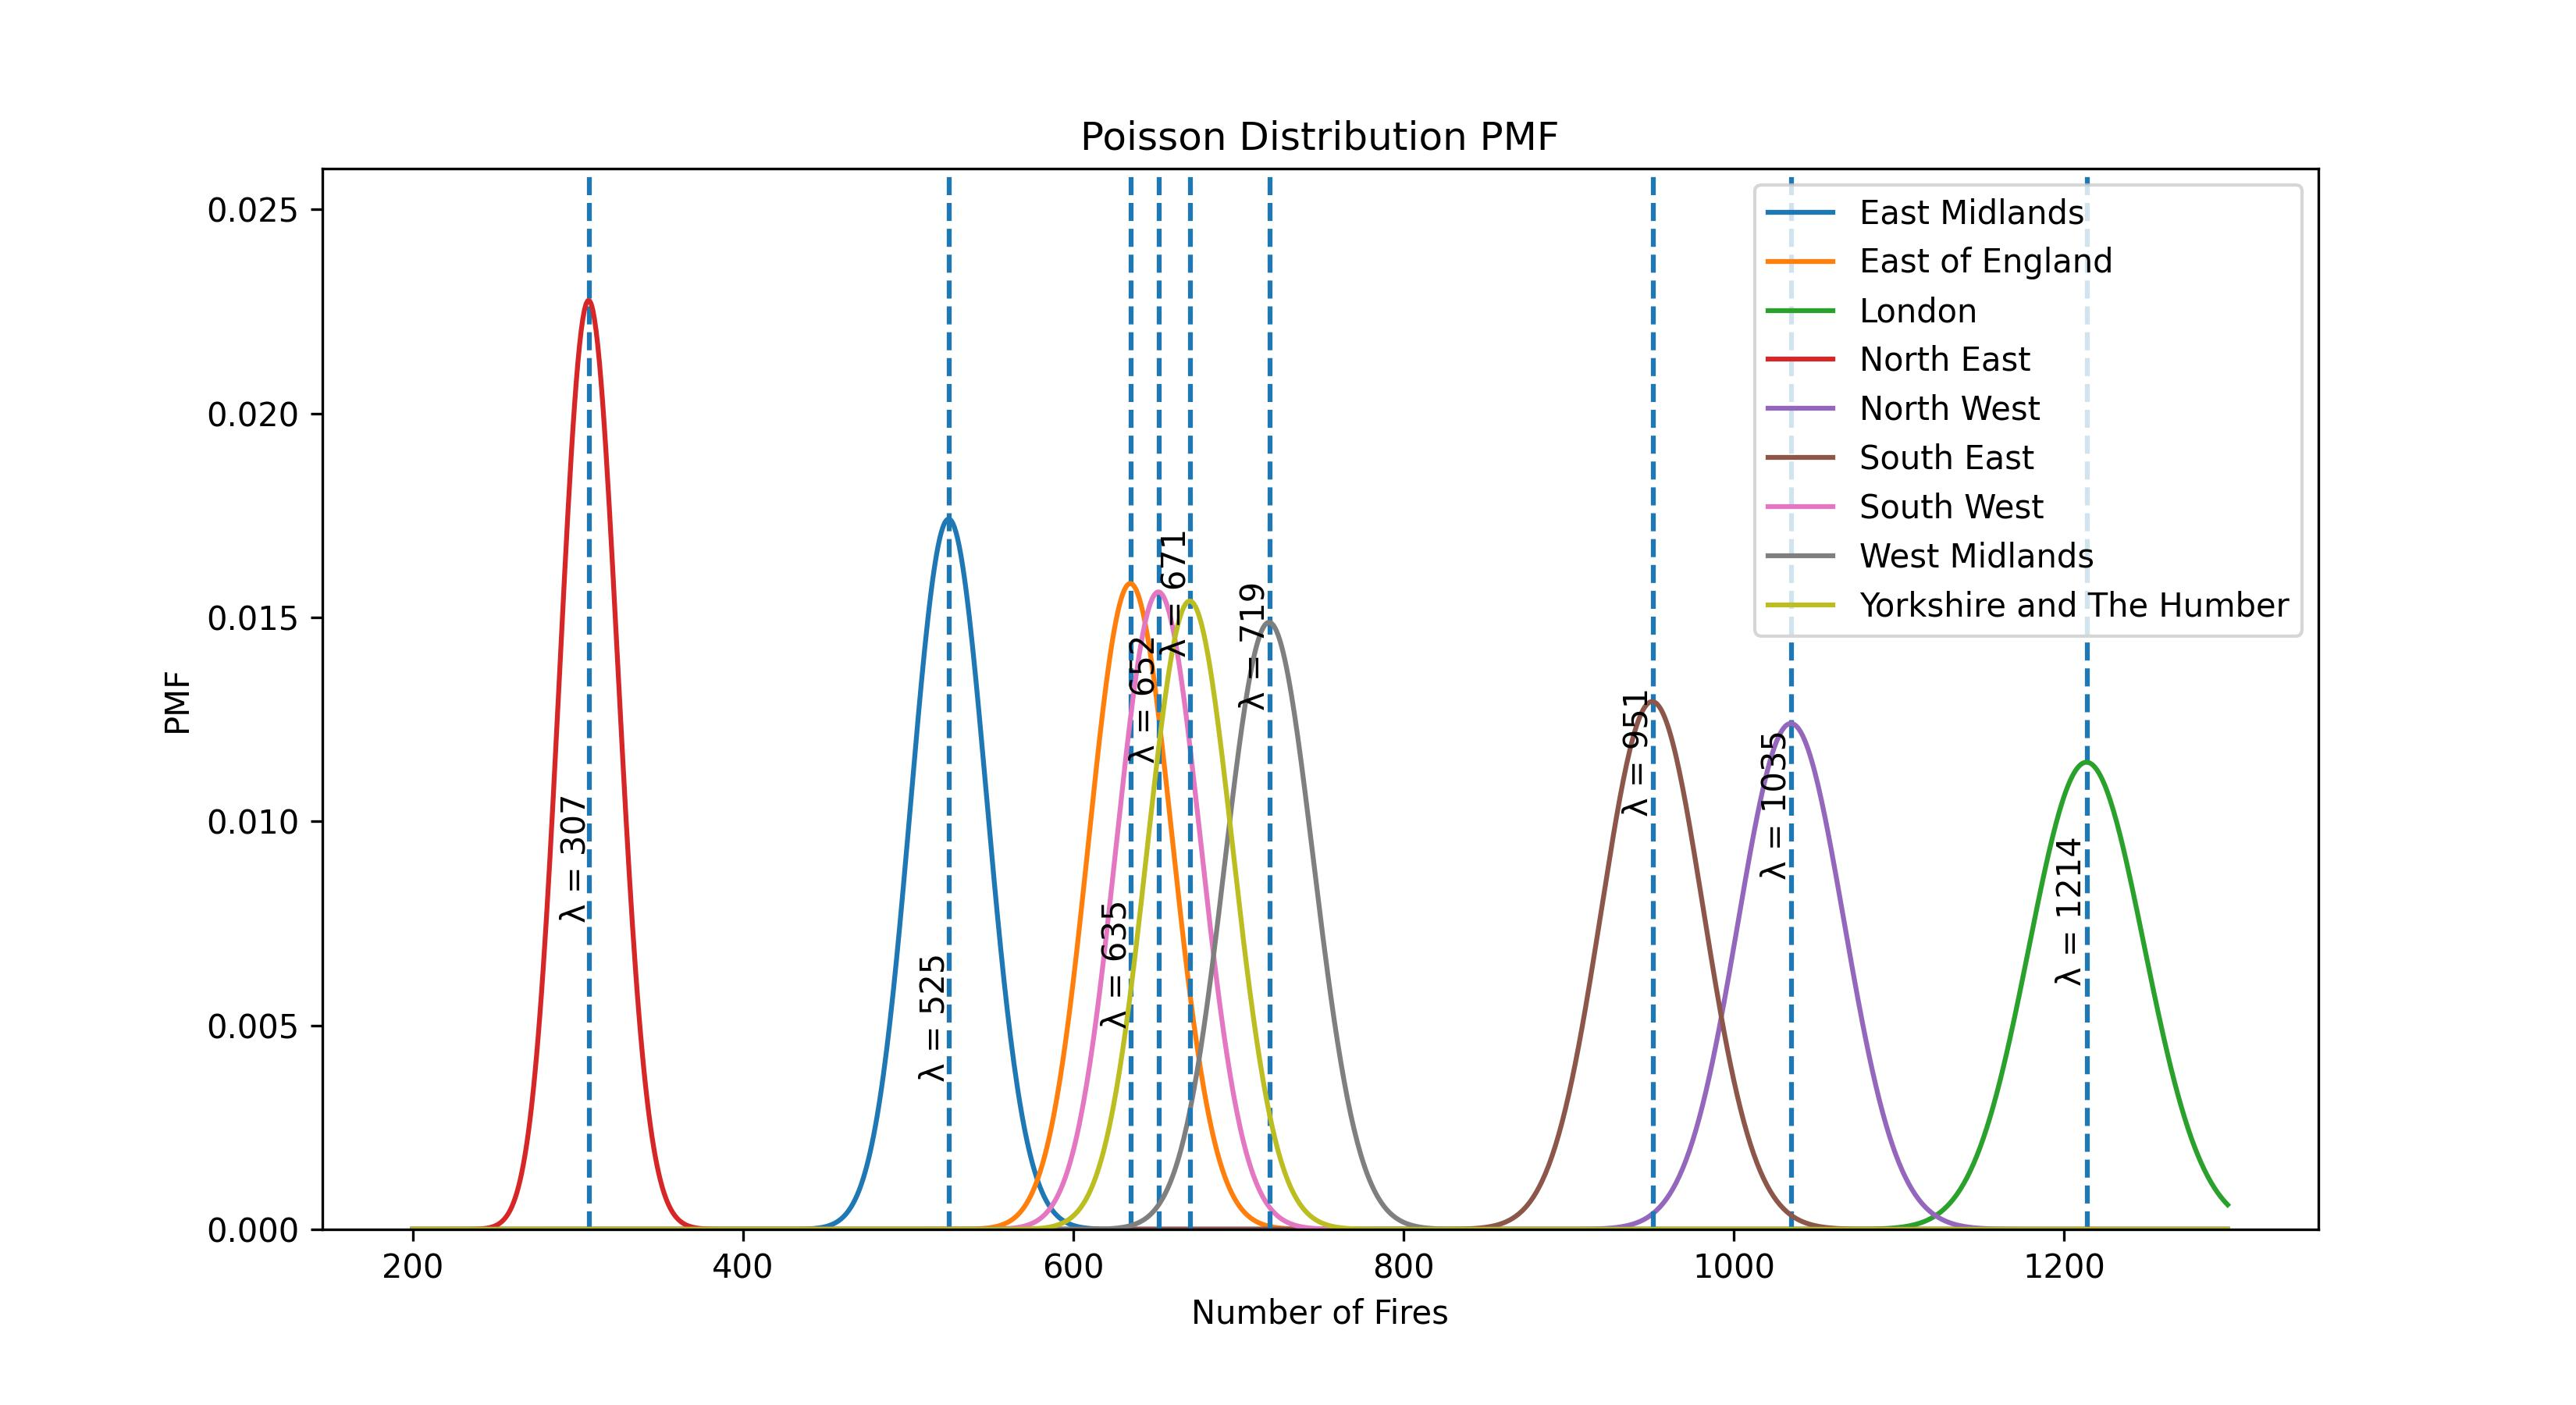
\includegraphics[width=\textwidth]{fire_dwell_times_pmf.jpg}
\caption{}\label{subfig:firedwell}
\end{subfigure}
\caption{Figure (\ref{subfig:fireall}) on the left shows the pmf of the exponential distribution of the number of 
fires in different areas, and Figure (\ref{subfig:firedwell}) on the right shows the pmf of the exponential distribution 
of the number of fires in dwelling in different areas}\label{fig:firepmf}
\end{figure}

\subsubsection{Details about Model of the Number of Fires Per Year}
The use of the Poisson distribution gives a good prediction of the number of fires per year.\textsuperscript{\cite{poisson, firepossion}}
The form of the Poisson distribution is given below:
\begin{equation}
    f(N ; \lambda)=\left\{\begin{array}{cc}
        \lambda e^{-\lambda N} & N \geq 0 \\
        0 & , N<0
        \end{array}\right.
\end{equation}

Given a sample of observations $N_1, N_2, ..., N_n$, we aim to find the maximum likelihood estimate of the parameter $\lambda$.

Firstly, the likelihood function $L(\lambda; N_1, N_2, ..., N_n)$ is the joint probability density of the observations, which is:

\begin{equation}
L(\lambda; N_1, N_2, ..., N_n) = \prod_{i=1}^{n}\lambda e^{-\lambda N_i}
\end{equation}

Because products are typically more complicated for optimization, we can take the logarithm of the likelihood function to get the log-likelihood function:

\begin{equation}
l(\lambda; N_1, N_2, ..., N_n) = \log L(\lambda; N_1, N_2, ..., N_n) = \sum_{i=1}^{n} \log (\lambda e^{-\lambda N_i}) = n\log\lambda - \lambda \sum_{i=1}^{n} N_i
\end{equation}

To solve for the optimal $\lambda$, we need to find the $\lambda$ that maximizes the log-likelihood function. So we take the derivative of $l(\lambda)$ with respect to $\lambda$, set it to zero and solve for $\lambda$:

\begin{equation}
\frac{\partial l(\lambda; N_1, N_2, ..., N_n)}{\partial \lambda} = \frac{n}{\lambda} - \sum_{i=1}^{n} N_i = 0
\end{equation}

From which we obtain:

\begin{equation}
\hat{\lambda}_{MLE} = \frac{n}{\sum_{i=1}^{n} N_i} = \frac{1}{\text{E}[N]}
\end{equation}

This gives us the maximum likelihood estimate of the parameter $\lambda$ in an exponential distribution.

\subsection{Annual Price Model for Claims Arising from Fire}

We will assess the distribution of claims due to fire each year. The results is shown in Figure (\ref{fig:max}). This problem can be decomposed in the following steps:

\textbf{Step 1: Determine the distribution of the total number of fires per year}

Based on the data provided, we already know the distribution of the number of residential fires per year, and we also know the proportion of residential fires to the number of all fires. Let the proportion be $R$ and $P_{\text{residential}}$ be the distribution of the number of dwelling fires per year, we can calculate the distribution of the total number of fires per year as follows $P_{\text{all}}$:

$$
P_{\text{all}} = \frac{P_{\text{residential}}}{R}
$$

Here, we make the important assumption that the number of residential fires per year as a proportion of the total number of fires is equal to the proportion of residential fire losses per year as a proportion of total fire losses. Although this assumption may not be entirely accurate, in the absence of other information, we will use this approach.

\textbf{Step 2: Determine the distribution of losses per fire}

Based on the known distribution of house prices (log-normal distribution), we can infer the distribution of losses from each fire. We assume that the loss per fire is proportional to the house price, and therefore the distribution of losses due to each fire can also be considered as a log-normal distribution.

\textbf{Step 3: Estimate the distribution of total losses due to fires per year}

With the distribution of the number of fires per year and the distribution of losses per fire known, we will apply Monte Carlo simulations\textsuperscript{\cite{MonteCarlo}} to estimate the distribution of the total losses due to fire per year.

\textbf{Step 4: Calculate the distribution of claims due to fire per year}

We also need to know the ratio between the annual fire losses and the claims. Setting $C$ as this ratio, we can then calculate the distribution of annual claims due to fire by using the following formula:

$$
\text{Claims\_distribution} = \text{Loss\_distribution} \times  C
$$

In summary, we first estimate the distribution of the total number of fires per year and the distribution of losses per fire by using some known distributions and assumptions. We then apply Monte Carlo simulations to estimate the distribution of the total losses due to fires per year. Finally, we calculate the distribution of claims due to fire per year based on the ratio between losses and claims


\subsection{Predict}
We have chosen to use the ARIMA model to forecast the key parameters for our estimate of annual fire losses. The ARIMA model is a commonly used model for forecasting time series.\textsuperscript{\cite{arima4, arima, arima2, arima3}}

\subsubsection{Introduction to the ARIMA model}

The ARIMA model, an acronym for Autoregressive Integrated Moving Average Model, is a commonly used model for describing univariate time series. The model combines the autoregressive (AR), differencing (I) and moving average (MA) models in an attempt to predict future values based on past values, error terms and trends in the time series.

In the ARIMA model, "AR" stands for "autoregressive", which predicts future observations based on a linear combination of past observations. "I" stands for "integrated", which makes the time series stationary by taking the difference once or several times. "MA" stands for "moving average", which predicts future observations based on a linear combination of past error terms.

The ARIMA model can be written as

\begin{equation}
\phi(B) (1-B)^d X_t = \theta(B) Z_t
\end{equation}

where $X_t$ is the time series, $B$ is the backward shift operator (i.e. $BX_t = X_{t-1}$), $d$ is the order of differencing, $Z_t$ is a white noise series, and $\phi(B)$ and $\theta(B)$ are polynomials in the backward shift operator.

\subsubsection{Forecasting Process}

Our prediction process is twofold. First, we use the ARIMA model to forecast key parameters, including the frequency of fires, the loss per fire, and the ratio of losses to claims, among others. Our forecasting results are detailed in Table \ref{tb:pred}.

We then feed the predicted parameters into our previously constructed model, calculate the distribution of annual fire losses using Monte Carlo simulation, and finally derive the predicted distribution of annual fire losses for 2023.

It's worth noting the limitations of the ARIMA model. The model assumes that the time series is stationary. If there are trends or seasonality in the series, we would need to pre-process the data, such as taking differences or applying a logarithmic transformation, to ensure stationarity. In addition, the ARIMA model is sensitive to the choice of parameters; inappropriate parameters can lead to significant deviations in the forecast results.

\begin{figure}
    \centering
    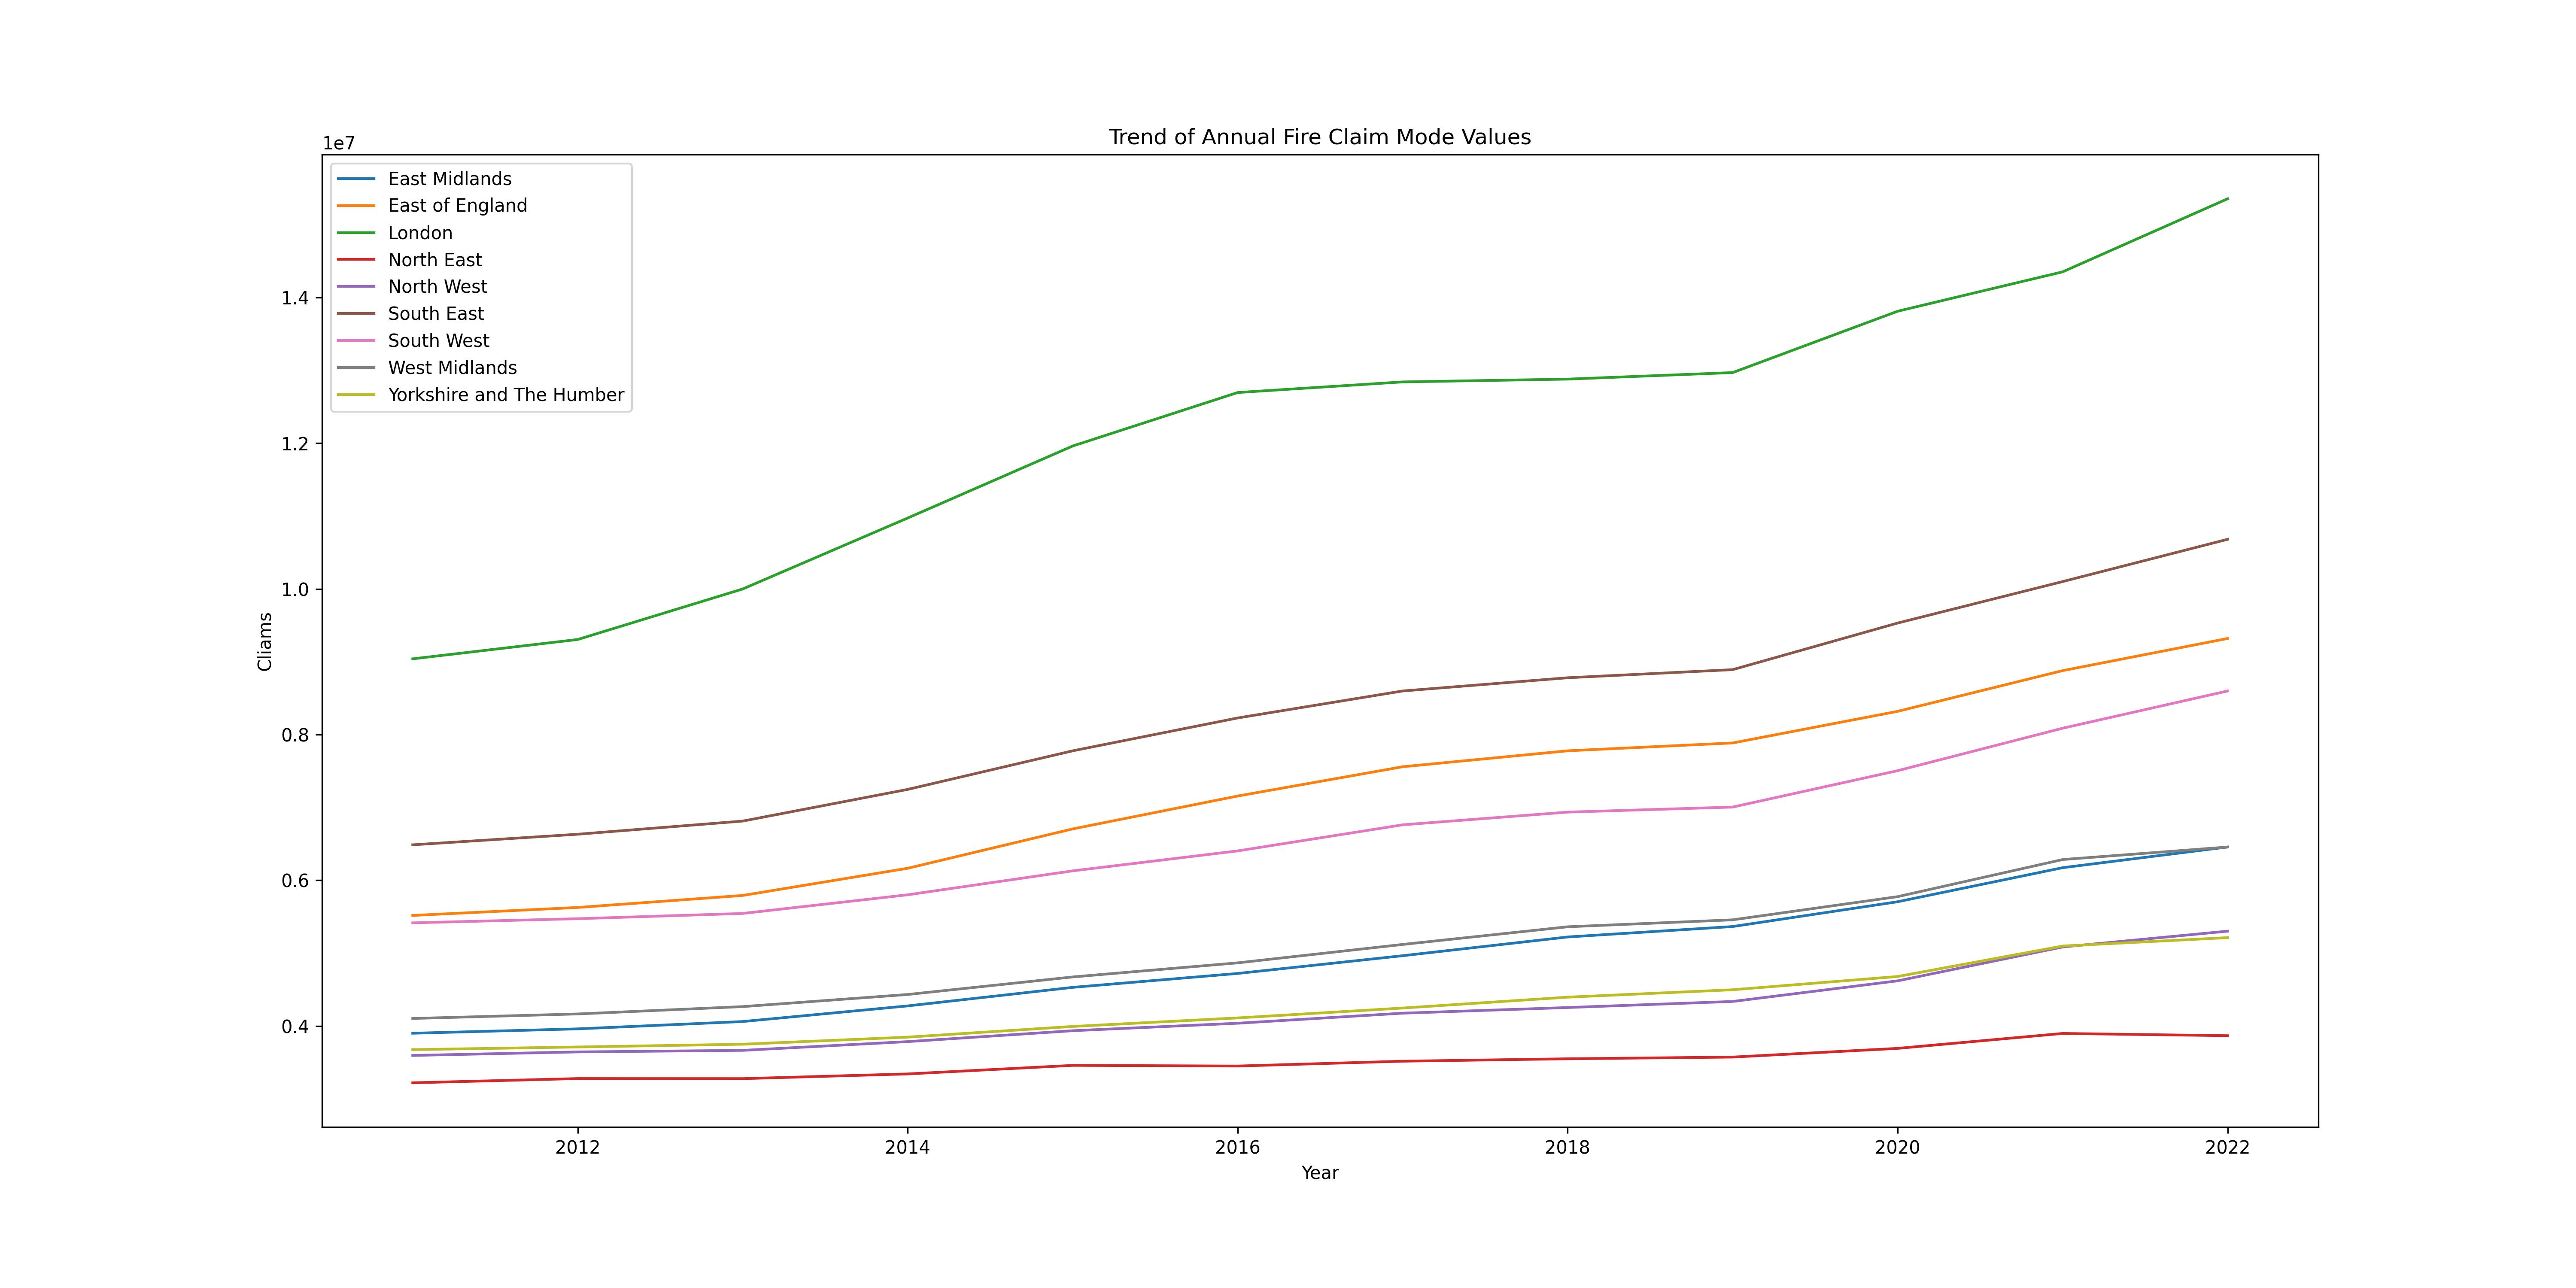
\includegraphics[width=\textwidth]{max.jpg}
    \caption{This graph shows the total amount of fire claims due to fires per year predicted by our model based on data from the past 9 years, using the model's most probable value.}\label{fig:max}
\end{figure}

\begin{table}[!htbp]
    \begin{center}
    \caption{2023 Predict Parameter}

    \begin{tabular}{ccccc}%四个c代表有四列且内容居中
        \toprule%第一道横线
        &\multicolumn{2}{l}{\textbf{\underline{\quad Log House Price \quad}}}& \textbf{\underline{Number of Fires}}&\\%跨两列;内容居中;跨列内容为Resultsummary通过\textbf{}与\underline{}命令分别对内容加粗、加下划线        
        Region&Mean&STD&Mean&CPI \\

        \midrule
        East Midlands&12.41746&0.57385&52744&\multirow{9}*{138.499}\\
        East of England&12.77447&0.65185&57558&~\\
        London&13.27747&0.76739&183921&~\\
        North East&11.87081&0.64632&56030&~\\
        North West&12.17349&0.58698&106850&~\\
        South East&12.93920&0.67526&98270&~\\
        South West&12.74061&0.64467&72537&~\\
        West Midlands&12.39147&0.59135&50056&~\\
        Yorkshire and The Humber&12.18806&0.64153&84288&~\\

        \bottomrule
    \end{tabular}\label{tb:pred}
    \end{center}
    \end{table}

\section{Summary}


\clearpage
\bibliographystyle{unsrt}
\bibliography{ref.bib}

\begin{subappendices}  % 附录环境

\section{Appendix A: Further on \LaTeX}
To clarify the importance of using \LaTeX\ in MCM or ICM, several points need to be covered, which are \ldots

To be more specific, \ldots

All in all, \ldots

Anyway, nobody \textbf{really} needs such appendix \ldots

\section{Appendix B: Program Codes}
Here are the program codes we used in our research.

% 代码环境示例三则
% 如您的论文不需要展示代码,请删除
% 更多用法,请参考 listings 宏包文档

% Python 代码示例
\begin{lstlisting}[language=Python, name={test.py}]
# Python code example
for i in range(10):
    print('Hello, world!')
\end{lstlisting}

% MATLAB 代码示例
\begin{lstlisting}[language=MATLAB, name={test.m}]
% MATLAB code example
for i = 1:10
    disp("hello, world!");
end
\end{lstlisting}

% C++ 代码示例
\begin{lstlisting}[language=C++, name={test.cpp}]
// C++ code example
#include <iostream>
using namespace std;

int main() {
    for (int i = 0; i < 10; i++)
        cout << "hello, world" << endl;
    return 0;
}
\end{lstlisting}

\end{subappendices}  % 附录内容结束

\end{document}  % 结束
% 三线表示例
% \begin{table}[!htbp]
% \begin{center}
% \caption{Notations}
% \begin{tabular}{cl}
%     \toprule
%     \multicolumn{1}{m{3cm}}{\centering Year}
%     &\multicolumn{1}{m{8cm}}{\centering Consumer Prices Index}
%     \\
%     \midrule
%     $2011$ &    {\centering 93.4}\\
%     $2012$ &96.1\\
%     $2013$ &98.5\\
%     $2014$ &100.0\\
%     $2015$ &100.0\\
%     $2016$ &100.7\\
%     $2017$ &103.4\\
%     $2018$ &105.9\\
%     $2019$ &107.8\\
%     $2020$ &108.7\\
%     $2021$ &111.6\\
%     $2022$ &121.7\\
%     \bottomrule
% \end{tabular}\label{tb:CPI}
% \end{center}
% \end{table}